\documentclass[10pt, onecolumn, draftclsnofoot, letterpaper, compsoc]{IEEEtran}

\usepackage{cite}
\usepackage{color}
\usepackage{hyperref}
\usepackage[normalem]{ulem}
\usepackage{enumitem}
\usepackage{minted}
\usepackage{graphicx}
\usepackage{geometry}
\usepackage{pdfpages}
\usepackage{tabularx}
\usepackage{longtable}

\graphicspath{ {resources/} }
\hypersetup{colorlinks=true, urlcolor=blue, linkcolor=black}
\geometry{textheight=8.5in, textwidth=7in}

%%%%%%%%%%%%%%%%%%%%%%%%%%%%%%%%%%%%%%%%%%%%%%%%%%%%%
% Macro for the signatures at the end                %
\newcommand*{\SignatureAndDate}[1]{%
    \par\noindent\makebox[2.5in]{\hrulefill} \hfill\makebox[2.0in]{\hrulefill}%
    \par\noindent\makebox[2.5in][l]{#1}      \hfill\makebox[2.0in][l]{Date}%
}%

\renewcommand*\contentsname{Table of Contents} % Rename ToC

\newcommand{\myindent}{\hspace{\oldparindent}}
% Temp title and author
\title{Final Report}
\date{\today} % Somehow this isn't working..
\author{Totality AweSun \\
		Bret~Lorimore, Jacob~Fenger, George~Harder \\
		\textit{\today \\
		Senior Capstone, Oregon State University}}

\begin{document}
\maketitle


\begin{abstract}

This document contains the final report summarizing the \textit{North American
Eclipse 2017} senior capstone project at Oregon State University. This
project is part of the larger Eclipse Megamovie Project. The Eclipse Megamovie
project is a citizen science project centered around the eclipse that will pass
over the United States on August 21st, 2017. It is a collaboration
between Google and scientists from UC Berkeley and several other institutions with the
aim of compiling a large dataset of eclipse observations. Acquiring coronal data
is of particular interest as the corona is not normally visible from Earth.
Specifically, the project will crowdsource photos of the eclipse from
photographers at various locations along the path of totality. These images will
be aligned spatially and temporally and stitched into a unique movie that shows
the eclipse over a period of 1.5 hours as it passes across the United States.
Additionally, the complete photo dataset will be open sourced so that
independent researchers may do their own analysis.

\end{abstract}

\vspace{10mm}
\noindent \SignatureAndDate{David Konerding, Project Sponsor}
\vspace{8mm}
\noindent \SignatureAndDate{Bret Lorimore}
\vspace{8mm}
\noindent \SignatureAndDate{George Harder}
\vspace{8mm}
\noindent \SignatureAndDate{Jacob Fenger}

\newpage

\tableofcontents

\newpage

% 1
\section{Introduction}
Bret interned at Google during the summer of 2016 where he worked on parts of
the Eclipse Megamovie Project. He asked his manager at the time,
David Konerding, to sponsor a capstone team to assist with the project.
Bret requested that the team consist of himself, George Harder, and Jacob
Fenger. Since Bret was familiar with the project from his internship, he
quickly molded into the technical expert of the group.
All of us worked on technical portions of the
project as well as ensuring the writing portions of the project were as good
as possible. David Konerding advised us on the development of the simulator,
processor, and developer pipeline while he was working on other aspects of the
Eclipse Megamovie Project.

% 2
\section{Requirements}

\subsection{Original Requirements Document}
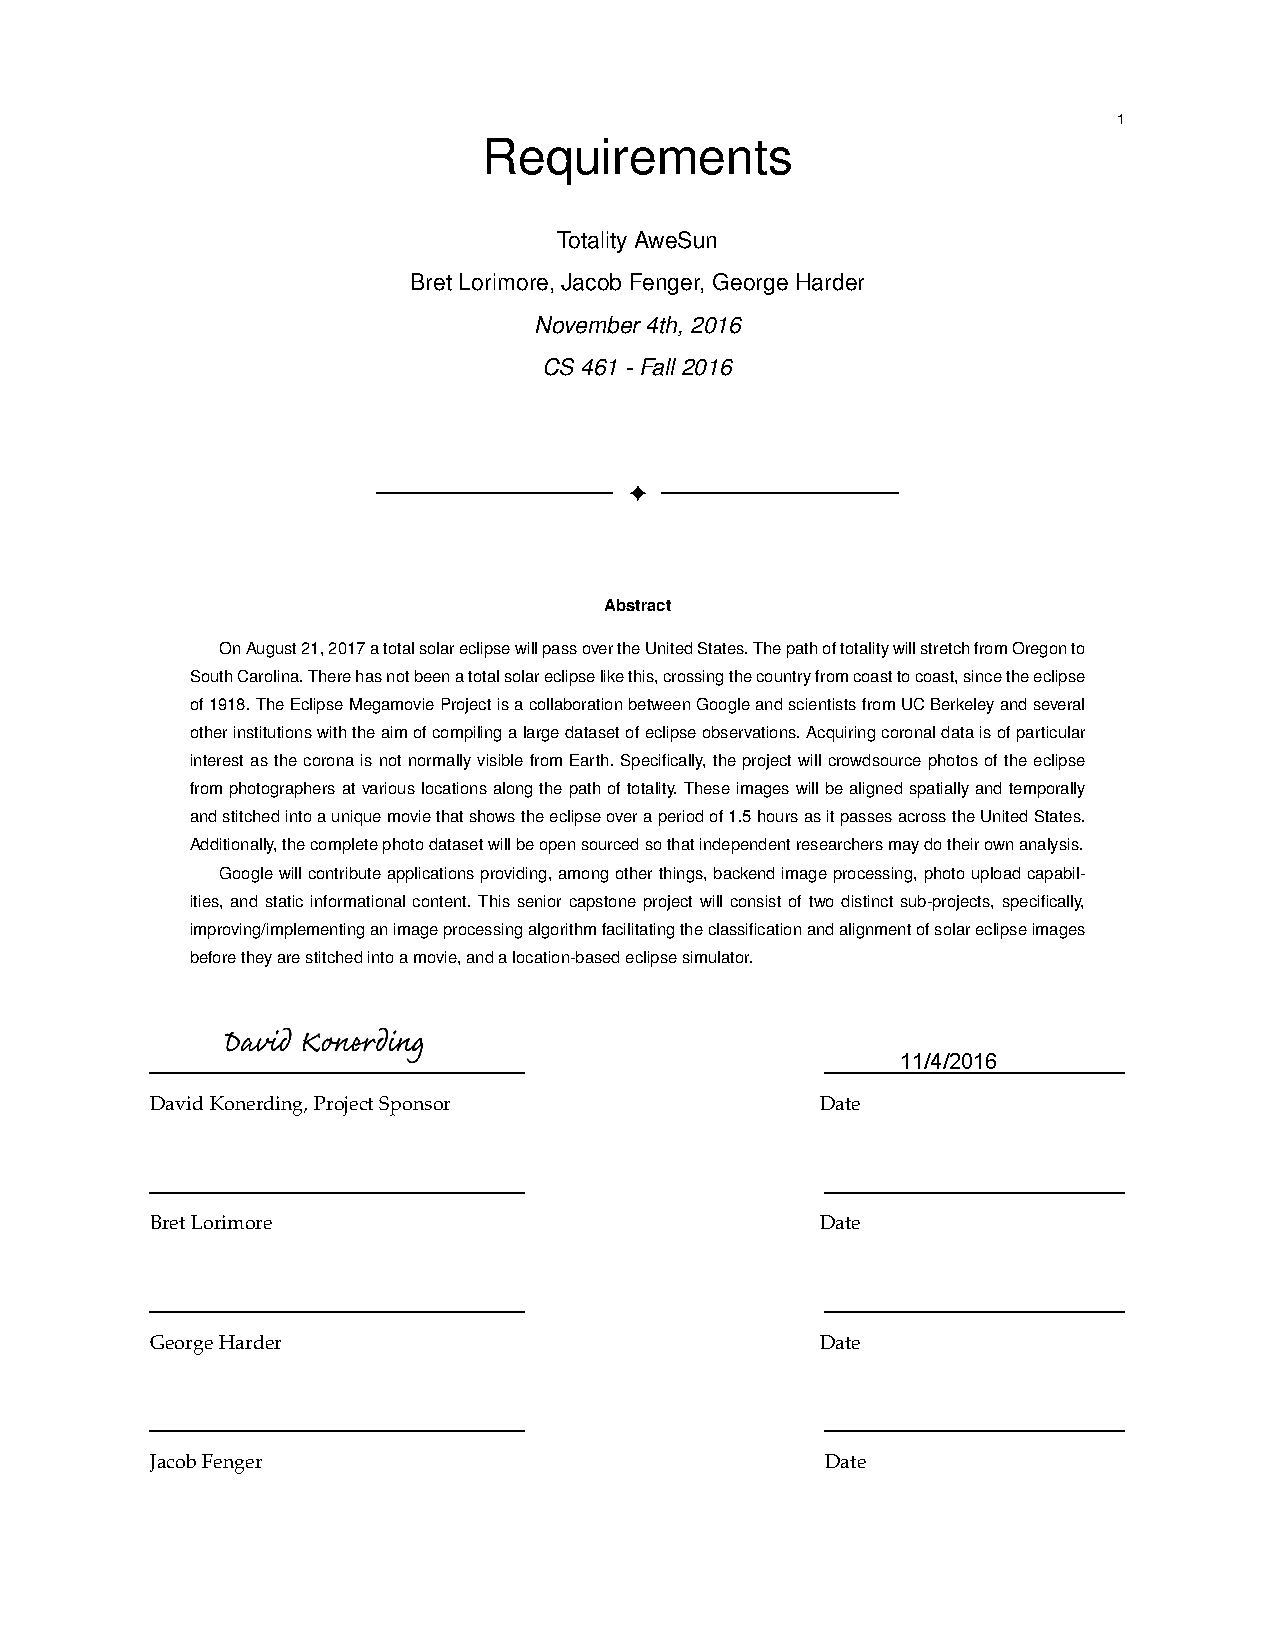
\includepdf[pages=-, frame, scale=0.8, pagecommand={}]{resources/reqs.pdf}

\subsection{Requirements Revisions}

\subsubsection{Requirements Changes}

\begin{longtable}{| p{.15\textwidth} | p{.25\textwidth} | p{.25\textwidth} | p{.25\textwidth} |}
\hline
\textbf{\# in Original Document} & \textbf{Requirement} & \textbf{Changes} & \textbf{Comments} \\ \hline

	% Bret
    3.1.1.3 &
	Users will be able to adjust the simulator time from 12 hours before
	the eclipse to 12 hours after it.
	\begin{enumerate}
		\item Time can be advanced via a draggable slider or clickable buttons.
	\end{enumerate} &
	Changed to 1.5 hours before / after the eclipse. &
	This change came from our UX designer and product manager, who felt that 12 hours created too much padding before / after the eclipse.
	\\ \hline

	3.1.2.1 &
	The image pre-processor will be compatible with Ubuntu 16.04 and will include a script that to install all dependencies/build the binary. &
	Changed so that we will include \textit{instructions} to install dependencies and a textit{makefile} to build the binary. &
	This allows for separation of dependency installation and building of the actual program.
	\\ \hline

	3.1.2.2 &
	The application will accept the following input as command line
	arguments:
	\begin{enumerate}
	   \item Required: image\_list\_file
		   \begin{enumerate}
			   \item Absolute or relative (to the directory the binary was
			   invoked from) path to file containing a list of image filenames
			   with no directory prefix.
		   \end{enumerate}

	   \item Required: output\_dir
		   \begin{enumerate}
			   \item Directory to write output files to.
		   \end{enumerate}

	   \item Optional: image\_path\_prefix
		   \begin{enumerate}
			   \item Absolute or relative (to the directory the binary was
				invoked from) path to prepend to each image filename in
				image\_file\_list. Defaults to "./".
		   \end{enumerate}
	\end{enumerate} &
	Removed image\_path\_prefix parameter and made it so that image\_list\_file must contain full paths.
	Added mode parameter. Added parameters for \texttt{cv::HoughCircles}. &
	image\_path\_prefix / image\_list\_file changes made at client's request, for convienience.
	Added parameters were added to improve image processor development workflow.
	\\ \hline

	3.1.2.4 &
	[Requirement too long, see original requirements document] &
	Renamed output file. Removed image crop / rotation / classification / EXIF based values.
	Added variable number of found circles, execution times, and general observations. &
	These changes were made as the overall goal of the image processor was simplified to
	simply recognize total solar eclipse position. Additionally, the format was made more
	flexible to aid in development of modified image processor pipelines.
	\\ \hline

	% George
    3.1.2.5 &
	Images that are rejected will not be added to the image transformations.txt file and will not be cropped/exported
    to the images directory. When an image is rejected a message with this information will be printed to stdout. &
	Removed &
	This requirement was removed because we never reached this stage in development of the image processor.
	\\ \hline

    3.1.2.6 &
    The application will format all log messages as follows:
    a) img preproc:level:timestamp:message
    i) Values of level: ERROR / WARNING / INFO / DEBUG
    ii) Value of timestamp: current timestamp
    iii) Value of message: specific logging message &
    Removed &
    This requirement was removed because our sponsor did not need logging built in to the image processor at this time.
    \\ \hline

    3.2.1.1 &
    Displayed solar/lunar placement will be based on location and time and will account for edge cases like
    when the location is not in the path of totality. For example, if the location is on the opposite side of the
    world as the eclipse, the simulator should shift to a night time display &
    Changed, the simulator is restricted to the United States so it does not need to account for cases around the world. &
    After discussions with our sponsor we agreed to restrict the simulator the US because that is the only place the
    eclipse is visible.
    \\ \hline

    3.2.1.2 &
    Simulator will display the local time that the simulator is set to, e.g. there is a well defined time associated
    with the user selecting Corvallis, Oregon as their location and a simulator time of -3:13 (3 hours 13 minutes)
    before the eclipse. This time should be displayed on the simulator. &
    Removed &
    This requirement was removed because our simulator ended up including a time slider that displayed local times
    relative to the eclipse so a standalone time display was unecessary.
    \\ \hline

    3.2.2.1 &
    Invalid JPEG and PNG files (e.g. cannot be opened by OpenCV, width/height equal to 0px, etc.) will be
    ignored and an error message will be written to stderr. &
    Removed &
    In discussions with our sponsor we decided that the image processor would only be handling valid images and
    as such would not need to identify invalid images and write and error message.
    \\ \hline

    3.2.2.2 &
    The application will classify the input images as being one of the following types:
    a) FULL DISK
    i) Image of an unobscured solar disk.
    b) TOTALITY
    i) Image of a total solar eclipse.
    c) CRESCENT
    9
    i) Image of a partially eclipsed Sun, creating a ”crescent” shape.
    d) DIAMOND RING
    i) Image of a nearly fully eclipsed Sun where there is one ”hot spot” on the Sun’s perimeter. This hot
    spot along with the Sun’s perimeter have the shape of a diamond ring. &
    Removed &
    Because of development constraints our sponsor decided that the image processor would only processes
    images of the eclipse at totality and ass such would not handle classification.
    \\ \hline

    3.2.2.3 &
    For images of type CRESCENT, the application will compute / export a delta of the position of the center
    of the Sun and the Moon relative to the size of the solar disk. This delta will be a signed value based on
    the Sun’s position, i.e. if the Moon is to the left of the Sun (in the cropped/rotated image) the delta will be
    negative and conversely, if the Moon is to the right of the Sun the delta value will be positive. &
    Removed &
    See explanation for requirement 3.2.2 2.
    \\ \hline

    3.2.2.4 &
    For images of type DIAMOND RING, the application will compute / export the size of the ”diamond”
    relative to the size of the solar disk. &
    Removed &
    See explanation for requirement 3.2.2 2.
    \\ \hline

	% Jake
    3.2.2.5 &
	Images where the solar disk has a radius of less than 50px will be rejected. &
	Removed &
	Ideal solar disk radius is subject to change and depends on the current
    image processor implementation.
	\\ \hline

    3.2.2.6 &
	The application will crop the images to be square with the Sun centered.
    The images will be cropped so that there is a 100px pad between the solar
    perimeter and the edge of the images on all sides. &
	Removed &
	Google will be handling the cropping of images and their respective ideal
    dimensions.
	\\ \hline

    3.2.2.7 &
    The application will rotate DIAMOND RING and CRESCENT type images so that
    they are aligned horizontally, as described by Krista et al. &
	Removed &
	Google will be handling the rotation of images.
	\\ \hline

    3.2.2.8 &
    For images with GPS EXIF information, the application will compute/export
    the percentage through the
    eclipse’s path of totality at which the image was taken. 0\% will be
    defined as the westmost point on that
    path of totality that is over land, this point is on the west coast of
    Oregon. 100\% will be defined as the
    eastmost point on the path of totality that is over land, this point is
    on the east coast of South Carolina.
    The application will compute the point on the path of totality nearest
    the point where the image was taken.
    This point will be used to compute the percentage through the path of
    totality at which the image was
    taken. &
	Removed &
	We do not handle any GPS EXIF informaion with the image processor. This will be done by Google.
	\\ \hline

    3.2.2.9 &
	Images with GPS EXIF information that are not on the path of totality will be rejected. &
	Removed &
	See above requirements comment.
	\\ \hline

    3.3.1.1 &
	All simulator resources will load in less than 500ms given a 1-10 Mbps internet connection. &
	Changed the loading time to 700ms. &
    This was changed due to client preferences.
	\\ \hline

\end{longtable}

\subsubsection{Requirements Additions}

\begin{longtable}{| p{.15\textwidth} | p{.385\textwidth} | p{.385\textwidth} |}
\hline
\textbf{\# in Latest Document} & \textbf{Requirement} & \textbf{Comments} \\ \hline

    3.1.1.4 &
	Users will be able to "play" the eclipse and advance through the available
    time domain automatically by pressing a play button. &
	Added to enhance user experience when visualizing the solar eclipse.
	\\ \hline

    3.1.2.2 &
	[Requirement too long, see original requirements document] &
	Additionally parameters were added when running the image processor to allow
    testing of different processing methods.
	\\ \hline

    3.1.2.4 &
    The application will write the following output to the output\_dir directory
    (When run in batch mode):
    a) metadata.txt
    i) File containing one line per image processed with the following values:
    A) processed\_image: processed image filepath (absolute)
    B) found\_circle(s): circles found by the image processor, format: c(center\_x, center\_y, radius)
    C) execution\_time(s): time(s) taken for varius parts of the image processor
    to execute, format t("name", num\_secs)
    D) observation(s): observations about the image, format, "observation text"

    b) Processed image files
    i) Processed image files will be saved into output\_dir &
    The purpose of the image processor changed as development began. These
    requirements changes reflect that change.
    \\ \hline

    3.1.3.1 &
    The developer pipeline will accept the following command line arguments:
    a) Required: \$DIR, the directory to use for the image/data storage. The
    following will be saved into DIR:
    i) If download flag set: A clone of the \$GCS\_BUCKET
    ii) A directory called output that will contain:
    A) All the processed images \$GCS\_BUCKET
    B) A metadata file that will contain the processed image names along with
    output information from the image processor
    C) An HTML file that includes summaries of the image processor output info. &
    The developer pipeline replaced the image processor manager. This was due to
    requirements changed by our sponsor.
    \\ \hline

    3.1.3.2 &
    Required: \$GCS\_BUCKET, the Google Cloud Storage Bucket that contains the image
    to process. &
    We utilize Google Cloud Storage Buckets for easy storage and access to
    eclipse images.
    \\ \hline

    3.1.3.3 &
    Optional: download, if set, the developer pipeline will download the images
    from Google Cloud Storage. Otherwise, it will assume these images are included
    in \$DIR/\$GCS\_BUCKET &
    See above requirement explanation.
    \\ \hline

    3.1.3.4 &
    Optional: \$PIPELINE\_FLAGS, arguments to pass to the image processor when
    it is involved. &
    See requirement 3.1.3.1 requirement explanation.
    \\ \hline

    3.2.1.2 &
	The simulator location will be restricted to the United States. &
	This requirement was added because the eclipse only occurs in the US so having the
    simulator function outside the US is not important.
	\\ \hline

    3.2.1.3 &
	The simulator environment will darken as the eclipse progresses. &
	This requirement was added because our sponsor requested it.
	\\ \hline

    3.2.1.4 &
    The simulator will feature a zoom mode, where the sun appears larger in the sky. In zoom mode, the sun
    will remain in the center of the screen. The simulator will effectively track along with the sun’s movement. &
	This requirement was added because our sponsor wanted to give photographers a close up
    view of the eclipse in the simulator.
	\\ \hline

    3.2.1.5 &
	The simulator will be mobile friendly. &
	This requirement was added by our sponsor since our simulator was going to be live on the web.
	\\ \hline

    3.2.2.1 &
    The image processor will be implemented as a class that will be easily inheritable / modifiable by
    developers. &
	This requirement was added by our sponsor to facilitate future image processor development.
	\\ \hline

    3.2.2.2 &
    The image processor will feature two modes, "window" and "batch". In window mode, after an image is
    processed, windows will open showing the original image, processed image, and intermediate images. In
    batch mode, all images will be processed sequentially without opening any windows. Processed images
    and metadata will be exported as described in External Interfaces: Eclipse Image Processor. &
	This requirement was added to facilitate development of the image processor.
	\\ \hline

    3.2.2.3 &
	The image processor will identify the circles of the sun/moon in the images it processes. &
	This requirement was added to clarify the functionality of the image processor.
	\\ \hline

    3.2.2.4 &
    The image processor will record the number of seconds (wall clock time) needed to complete various
    portions of each image’s processing. &
	This requirement was added so that we could monitor and improve the performance of the image processor.
	\\ \hline

    3.2.3.1 &
	The developer pipeline will be able to download images from Google Cloud Storage, if requested. &
	This requirement was added so that the pipeline can use many different datasets.
	\\ \hline

    3.2.3.2 &
    The developer pipeline will build and invoke the image processor on the requested images using batch mode. &
	This requirement was added so that the pipeline runs over entire image sets.
	\\ \hline

    3.2.3.3 &
    The developer pipeline will assemble the results of running the image processor into and HTML file. This
    HTML file, along with the processed images it references, will be uploaded to Google Cloud Storage to a
    public URL. &
	This requirement was added so that the image processor's results are easily viewable by a team of developers.
	\\ \hline

    3.2.3.4 &
    The HTML file created by the developer pipeline will summarize the data included in the metadata.txt file
    exported by the image processor. &
	This requirement was added so that the image processor's results are easily viewable by a team of developers.
	\\ \hline

    3.3.3.1 &
    The image processor developer pipeline will download/upload images from/to Google Cloud Storage in parallel. &
	This requirement was added so that the developer pipeline efficiently downloads photos.
	\\ \hline

\end{longtable}

\subsubsection{Final Gantt Chart}
\vspace{2mm}
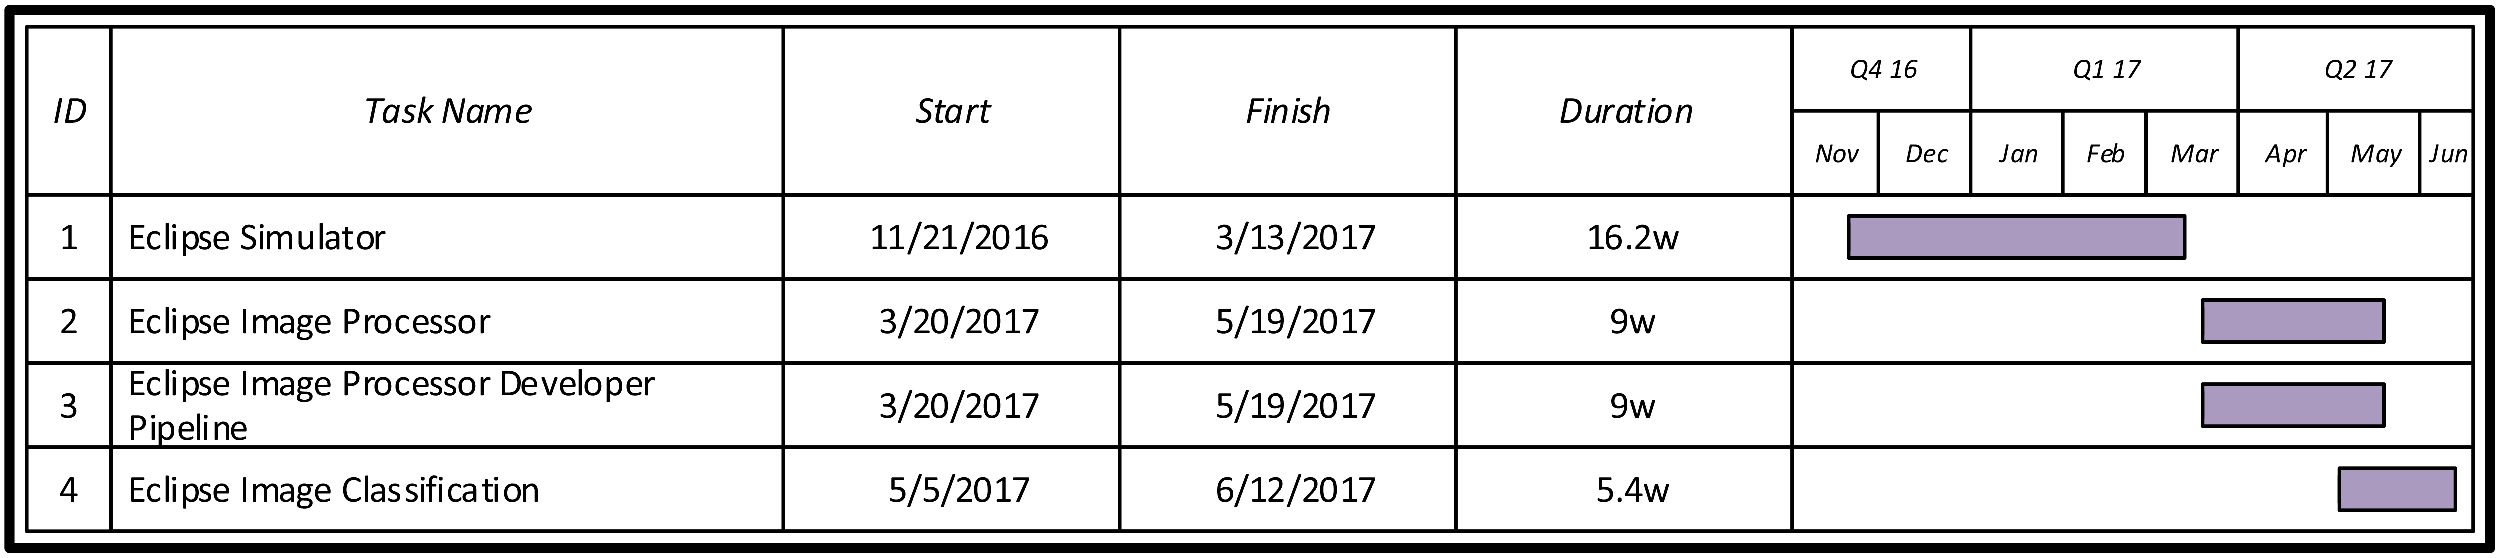
\includegraphics[width=\textwidth]{finalganttchart.pdf}

% 3
\section{Design Document}

\subsection{Original Design Document}
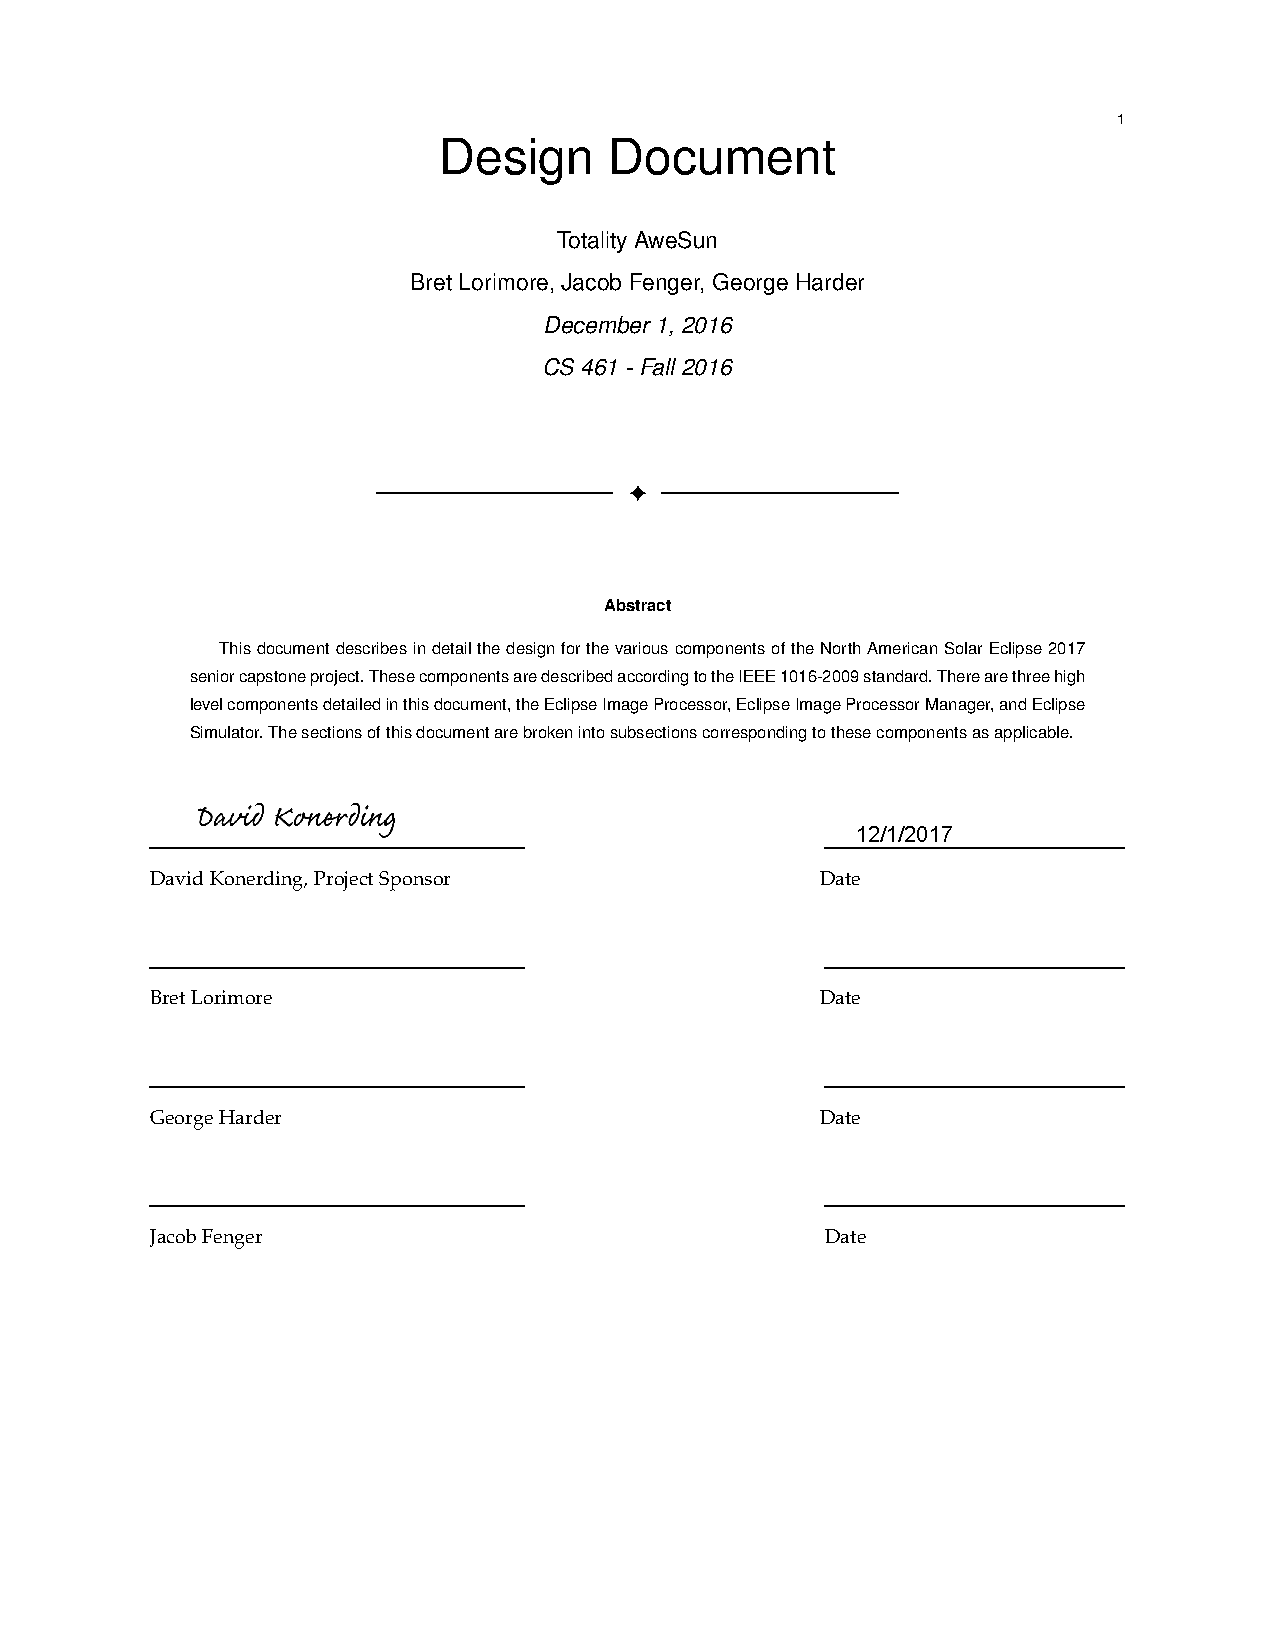
\includepdf[pages=-, frame, scale=0.8, pagecommand={}]{resources/design_doc.pdf}

\subsection{Design Document Changes}

Over the course of the year our design document changed significantly for several reasons.
First, our priorities shifted from image processing to building a fully featured and
robust simulator. Second, we had to scale back our initial goals for the image processor
and in response to delays in Google allowing code to be open sourced. Third, we
completely eliminated the image processor manager because of the combination of the
two previously mentioned factors. Lastly, we added a developer tool to the image processor
to facilitate further development after we left the project. This came about because as
our priorities shifted away from image processing and development time waned, we wanted to
make it easy for our sponsor to take over the development once we finished. The reasons for
all of these changes can be summed up as real world challenges that are to be expected over
the life of a project.

% 4
\section{Tech Review}

\subsection{Original Tech Review}
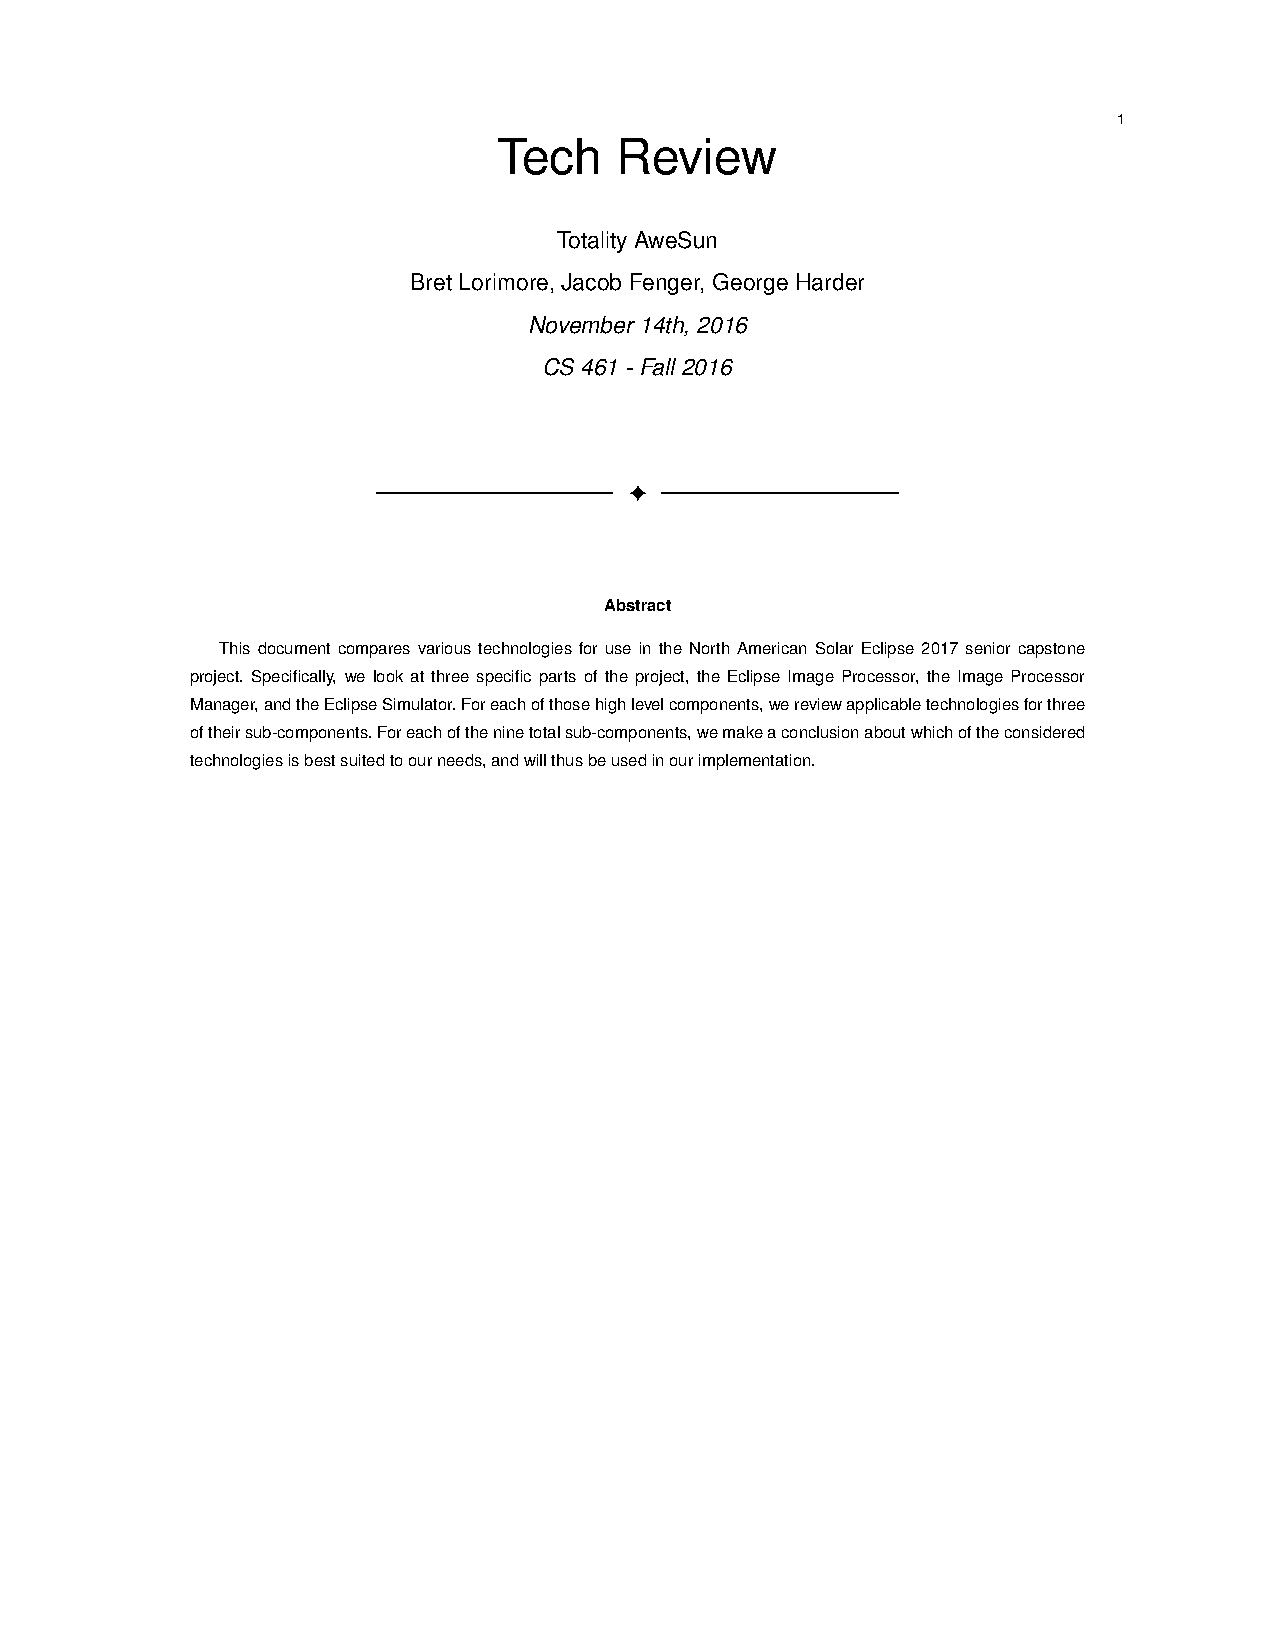
\includepdf[pages=-, frame, scale=0.8, pagecommand={}]{resources/tech.pdf}

\subsection{Tech Review Changes}
Before starting on the simulator, we chose a library called SunCalc for our
ephemeris computations.
During work on the eclipse simulator, we found that the ephemeris
computations were not very accurate and a library called Ephemeris provided
better results. As development increased, we realized again that Ephemeris
was not as accurate as we needed it to be. We looked to find another existing
library that provided more accurate results and found a library called
MeeusJs. This library is much more accurate and is used in the final simulator
version found on \href{https://eclipsemega.movie}{eclipsemega.movie}.

% 5
\section{Blog Posts}

\subsection{Fall Week 3}

    \subsubsection{Jake}

    \noindent \textbf{Jacob Fenger's Update 1}

    Week 3 is wrapping up and this will be the first update for our senior capstone
    project (CS 461) for fall term.

    \noindent \textbf{Plans for the upcoming week}

    Next week we will be having our weekly meeting with our client as well as our
    first meeting with our TA for the course of the school year, Vedanth Narayanan.

    \noindent \textbf{Progress Since Last Week}

    This week, we completed our project abstract as well as have gotten our
    document signed by our client. This github repo was also created to be used
    for our project.

    \noindent \textbf{Problems Encountered}

    No problems have been encountered so far in our project.

    \subsubsection{Bret}

    \textbf{Progress}

    Iterated on project statement following feedback from our sponsor and Kirstin.

    \noindent \textbf{Problems}

    None

    \noindent \textbf{Plans}
    \begin{itemize}
        \item We actually included a large amount of the content needed for the technology
        review in our initial project statement draft, so we will incorporate that
        into the Technology Review once that assignment is published.
        \item Talk with McGrath about somewhat unique characteristics of our project,
        follow up with our sponsor following this conversation.

    \end{itemize}

    \subsubsection{George}

    \noindent \textbf{Plans for the coming week}

    As of right now I have two important items on the agenda for next week. First,
    Bret and I plan to find Kevin in his office on Monday to discuss some time
    frames our project sponsor has in mind for the work and how those lineup with
    deadlines and due dates for the capstone class. Second, we have our weekly meeting
    with the project sponsor on Tuesday. We plan to ask what the sponsor would like
    in terms of us adding him to the Github repo and to discuss the conversation
    Bret and I have with Kevin.

    \noindent \textbf{Progress during this week}

    This week was spent working on and revising our project statement. We drafted
    the statement on Sunday, went over it with our sponsor on Tuesday, and met
    with Kirsten for feedback on Wednesday. Our final draft was successfully
    signed and turned in.

    \noindent \textbf{Problems Encountered}

    Being in the early stages of the project we have not yet encountered any significant difficulties.

\subsection{Fall Week 4}

    \subsubsection{Jake}

    \noindent \textbf{Plans for the upcoming week}

    Next week we will be finalizing and sending our revised problem statement to
    our client for it to be signed. We will also be having a meeting on Tuesday
    with him to discuss requirements of our project. Our meeting with our TA is
    Monday as well. George, Bret, and I will also be meeting to draft a requirements
    document that will be due next Friday.

    \noindent \textbf{Progress Since Last Week}

    This week, we revised our problem statement document. In addition, I have
    worked a little bit on image processing with OpenCV in C++. I worked on applying
    a Sobel filter to images which is used for edge detection. OpenCV makes this very easy to do.

    \noindent \textbf{Problems Encountered}

    No problems have been encountered so far in our project.

    \subsubsection{Bret}

    \noindent \textbf{Plans for the coming week}

    This week we will be completing revisions on our problem statement, getting
    it signed by @dakoner, and turning it in. Additionally, we will be working
    on our requirements document. I feel like we have a pretty good grasp on the
    requirements from a high level, but we will need to discuss them in detail with
    @dakoner in our call on Tuesday.

    \noindent \textbf{Progress this week}

    This week we synced with @dakoner regarding progress of the Google team and
    reviewed rotation matrices/researched quaternions at his suggestion. We also
    had our initial meeting with our TA which went very well. I am looking forward
    to working with him as we complete the rest of the project.

    \noindent \textbf{Problems Encountered}

    I did not think we encountered any problems/blockers this week.

    \subsubsection{George}

    \noindent \textbf{Plans for the coming week}

    Next week we have several items on the agenda. First, we will have our weekly
    update with our TA, Vedanth, on Monday at 2:00. After that we are going to meet
    back up a little later in the afternoon to start work on our Requirements
    Document. Lastly, we have our weekly update meeting with our project sponsor on Tuesday.

    In addition to these meetings, we are going to get our revised Problem Statement
    signed by our project sponsor. Currently the plan is to have it in his inbox by
    Monday morning so it is ready to be turned in Wednesday.

    \noindent \textbf{Progress this week}

    This week we received and incorporated feedback from the instructors on our
    problem statement. On Friday afternoon, we met as a group to discuss the feedback
    we received and incorporate revisions into the document.

    \noindent \textbf{Problems Encountered}

    Fortunately, we still have yet to encounter any significant blocking issues
    on this project.

\subsection{Fall Week 5}

    \subsubsection{Jake}

    \noindent \textbf{Plans for the upcoming week}

    Next week, we will be finishing up our requirements document as well as
    getting it signed by our client. Additionally, we will be meeting with our
    TA, Vedanth, as well as our client. We will continue to solidify our requirements,
    especially when it comes to classifying images once we have properly aligned them.

    \noindent \textbf{Progress Since Last Week}

    This week, we finished up the revised edition of our problem statement. We
    have also created a draft of the requirements document which will be turned in today.

    \noindent \textbf{Problems Encountered}

    No problems have been encountered so far in our project.

    \subsubsection{Bret}

    \noindent \textbf{Plans for the coming week}

    Next week we need to revise the initial draft of our requirements document,
    review this with @dakoner, make any changes he requests, and then get it signed
    by him/turn it in.

    \noindent \textbf{Progress this week}

    This past week we met with @dakoner, discussed the requirements document from
    a high level, and created an initial draft of this document.

    \noindent \textbf{Problems Encountered}

    No problems encountered this week.

    \subsubsection{George}

    \noindent \textbf{Plans for the coming week}

    Next week we have our two weekly meetings, one with our TA and one with our
    project sponsor. At these meetings we hope to discuss the draft of our requirements
    document and receive feedback on it. After these meetings we will revise our
    requirements document and prepare to turn it in.

    \noindent \textbf{Progress this week}

    This week our primary push was on a draft of the requirements document. Our
    first draft is completed and we are going to turn that in today, Friday 10/28.

    \noindent \textbf{Problems Encountered}

    We do not have not encountered any problems.

\subsection{Fall Week 6}

    \subsubsection{Jake}

    \noindent \textbf{Plans for the upcoming week}

    Next week, we will be meeting our client to catch him up with the current
    status of our project. Additionally we will be meeting with Vedanth, our TA,
    to discuss our plans as well. We will soon get started with implementing some
    aspects of our project, such as circle detection for eclipse images.

    \noindent \textbf{Progress Since Last Week}

    This week, we finished up the requirements document and turned it in. We also
    received feedback regarding our problem statement, which was very helpful.

    \noindent \textbf{Problems Encountered}

    No problems have been encountered so far in our project.

    \subsubsection{Bret}

    \noindent \textbf{Plans for the coming week}

    \begin{itemize}
    \item Begin work on the technical report assignments.
    \item Connect with @dakoner regarding the status of open sourcing the existing codebase.
      Also need to ask about getting ahold of JavaScript code to calculate solar/lunar position based
      on location. @dakoner has said he has this and we will need it for the eclipse simulator - I do
      not think it will be part of the open source release of the rest of the code.

    \end{itemize}

    \noindent \textbf{Progress this week}

    \begin{itemize}
    \item This week we met with @dakoner who reviewed our requirements document and was happy with the
      requirements we'd come up with.
    \item Following a request last week from @dakoner for the Eclipse Image Processor to use GPS EXIF info
      when available, we proposed a scheme to do this which @dakoner was happy with. We incorporated this
      into our requirements document.
    \item @dakoner shared our requirements with another Google engineer who is working on seperate part of the
      project. This is exciting and means we really will need to stick to the requirements as stated in our
      document.

  \end{itemize}

    \noindent \textbf{Problems Encountered}

    No problems encountered this week.

    \subsubsection{George}

    \noindent \textbf{Plans for upcoming week}

    Next week we will likely begin working on the technical review assignment.

    \noindent \textbf{Progress this week}

    This week was consumed with getting the requirements document written. We met
    a couple times to work on and finalize the requirements document. I focused on
    the first two sections, however, I added to the third section.

    \noindent \textbf{Challenges encountered}

    So far we have not encountered any challenges.

\subsection{Fall Week 7}

    \subsubsection{Jake}

    \noindent \textbf{Plans for the upcoming week}

    \begin{itemize}

    \item Meet with our TA, Vedanth, on Monday
    \item Meet with our client on Tuesday
    \item Begin work on JavaScript simulator. Will most likely use SVG from HTML5 for
    graphics/animation.

    \end{itemize}

    \noindent \textbf{Progress Since Last Week}

    This week, we met with our client regarding some additional project components.
    Additionally, he sent us some JavaScript code for computing the positions of the
    Sun and Moon at a given time/location. This utilizes some JavaScript back-end
    libraries called "Ephemeral" and "SunCalc".

    \noindent \textbf{Problems Encountered}

    We received some additional requirements regarding the collection of solar eclipse
    images to be processed. We talked about this requirement and it does not add too
    much to our project for us to be worried about.

    \subsubsection{Bret}

    \noindent \textbf{Plans for the coming week}

    \begin{itemize}

    \item Begin work on design document.
    \item Begin work on JavaScript eclipse simulator. This will include the UI and solar/lunar position calculations.

        \begin{itemize}
            \item Use code provided by @dakoner as reference/starting point.
        \end{itemize}

    \item Revise requirements document based on call with @dakoner this week. We are picking up an additional project
      component, an application that collects/downloads user uploaded eclipse images to be processed by the image
      processor application, invokes the image processor with these images as input, and collects the output of the
      image processor application and uploads it to Google Cloud.

    \end{itemize}

    \noindent \textbf{Progress this week}

    \begin{itemize}

    \item Met with @dakoner, where he expressed a desire for us to pick up the additional project component listed above.
    \item Acquired JavaScript code from @dakoner which computes altitude/azimuth of the Sun/Moon based on a
      latitude/longitude and date/time.

    \end{itemize}

    \noindent \textbf{Problems Encountered}

    I was initially hesitant about picking up the extra project component listed above. After realizing that it
    is very similar to some work I did at my internship this summer I felt better about this. Once that work is
    open sourced by @dakoner, we will be able to base this new component heavily on this previous work. Our group
    talked all this over after the meeting with @dakoner and we feel confident that we can take on this extra
    project component.

    \subsubsection{George}

    \noindent \textbf{Plans for the coming week}

    Next week we have our two weekly meetings, one with our TA and one with our
    sponsor. In addition to these, we need to turn in our technical review by the
    end of the day Monday. After these, we will likely begin discussing plans for
    the design document.

    \noindent \textbf{Progress this week}

    This week we focused on the technical review. We met during the week to divide
    up the pieces and technologies that we would be responsible for. After that,
    we individually worked on writing up the parts of the tech review.

    \noindent \textbf{Problems Encountered}

    We have not encountered any problems.

\subsection{Fall Week 8}

    \subsubsection{Jake}

    \noindent \textbf{Plans for the upcoming week}

    \begin{itemize}

    \item Meet with our TA, Vedanth, on Monday
    \item Meet with our client on Tuesday
    \item Continue work on the Eclipse Simulator. Look utilizing the Python "Ephem" library
     for computing the time of a solar eclipse for a given location.

    \end{itemize}

    \noindent \textbf{Progress Since Last Week}

    \begin{itemize}

    \item Began work on Eclipse Simulator

        \begin{itemize}
           \item Looked at computing altitude and azimuth using the SunCalc and Ephemeris libraries
           \item Wrote code to detect the time of a solar eclipse given a solar eclipse (Uses Python Ephem library)
       \end{itemize}

    \item Finished tech. review
    \item Began to work on the design document

    \end{itemize}

    \noindent \textbf{Problems Encountered}

    We initially found some problems when utilizing the Ephemeris JavaScript
    library. When comparing the SunCalc and Ephemeris library, it seemed that the
    Ephemeris library's computations were taking much longer than SunCalc's. Due to
    poor documentation, our client helped us realize that the functions in Ephemeris
    were expecting GMT times while we were just utilizing the local time. This made a
    huge different when computing the altitude and azimuth of the sun/moon at a given
    location/time.

    \subsubsection{Bret}

    \noindent \textbf{Plans for the coming week}

    \begin{itemize}

    \item Work on design document.
    \item Revise requirements/tech review based on updated requirements from @dakoner.
    \item Continue work on eclipse simulator.

    \end{itemize}

    \noindent \textbf{Progress this week}

    \begin{itemize}

    \item Met with @dakoner, discussed computations for the eclipse simulator, specifically regarding how to.
      determine eclipse time for a given location. This is the time that the simulator will initialize to.
    \item Began working on eclipse simulator.

    \end{itemize}

    \noindent \textbf{Problems Encountered}

    \begin{itemize}

    \item Running into some issues computing eclipse time for a given location. @dakoner sent over some Python
      code that can do this accurately, we have been unable to reproduce this entirely with JavaScript yet though.
      We are working on converting the horizontal parallax of the moon to angular size right now.
    \item We have also been running into some issues with inconsistent computations between SunCalc and Ephemeris JS.
      We are currently investigating these issues.

    \end{itemize}

    \subsubsection{George}

    \noindent \textbf{Plans for the coming week}

    This week we are going to begin work on the design document. In addition we
    have our usual weekly meetings.

    \noindent \textbf{Progress this week}

    This week we made major progress in completing the technical review. Each of
    us spent a fair amount of time researching different technologies that we could
    use to implement different features of our project. In addition Bret and I
    began to plan out how we would build the simulator.

    \noindent \textbf{Problems Encountered}

    We have not encountered any problems.

\subsection{Fall Week 9}

    \subsubsection{Jake}

    \noindent \textbf{Plans for the coming week}

    This next week will be finishing our design document, and making sure our
    client has seen it and has signed it for submission. In addition, we need to
    finish updating our requirements document as some of our requirements have
    changed recently. While we will be removing some requirements, we also need
    to add some. This won't cause many problems for us in terms of workload as
    everything is still pretty much the same. We will also need to plan how we
    want to do the final presentation. We will most likely use Powerpoint for the
    slides, and some sort of recording software/microphone to talk over them.

    \noindent \textbf{Progress this week}

    This past week, we met up to finalize what we were going to do for the design
    document. We had a little trouble understanding the IEEE standard we need to
    use but it should not be a problem.

    \noindent \textbf{Problems Encountered}

    We found some discrepancies regarding accuracy using the SunCalc/Ephemeris libraries
    and are continuing to work on these parts of the simulator to ensure everything is
    scientifically accurate.

    \subsubsection{Bret}

    \noindent \textbf{Plans for the coming week}

    \begin{itemize}

    \item Present initial design document draft to @dakoner, revise based on feedback as necessary.
    \item Create design document final draft.
    \item Revise requirements document based on recent requirement changes.
    \item Continue work on simulator - use existing percent eclipse computations to implement function that
      determines eclipse time for a given location.
    \item Begin thinking about final report and presentation.

    \end{itemize}

    \noindent \textbf{Progress this week}

    \begin{itemize}

    \item Synced as a group on high level design for project components - that way we are on the same page for the
      design document and can asynchronously work on our individual components.
    \item Will complete my part of design document this weekend.

    \end{itemize}

    \noindent \textbf{Problems Encountered}

    Ran into some issues with accuracy of eclipse percentage computation using Ephemeris JavaScript. @dakoner
    said he thinks we are accurate enough for the time being as this value is used to compute eclipse time - the
    initialization time for the eclipse simulator. This means that a <2 minute difference (which is where we're
    currently at) will not be noticeable.

    \subsubsection{George}

    \noindent \textbf{Plans for the coming week}

    This week I plan on working on the design document. My goal is to have my portion
    of the design document finished by Sunday night so that my team members can
    have a chance to review and revise the document as needed. In addition it will
    give us a chance to put all of our individual pieces together before we meet
    with our client on Tuesday and ask him to sign it.

    \noindent \textbf{Progress this week}

    This week we met a few times to go over what we wanted the design document to
    look like and to actually do some work on high level designs. These meetings
    were important because they gave us all a chance to think through design schemes
    and got us going in the right direction for writing the design document.

    \noindent \textbf{Problems Encountered}

    The only problem we had early in the week was trying to understand the format
    of the design document. How ever we talked in person with Kevin after class
    and now have a good idea of what to do.

\subsection{Fall Week 10}

    \subsubsection{Jake}

     \noindent \textbf{Plans for the coming week}

     \begin{itemize}

    \item Finish progress report document by Sunday
    \item Finish PowerPoint slides for progress report presentation by Monday
    \item Record progress report presentation
    \item Continue progress on eclipse simulator

    \end{itemize}

     \noindent \textbf{Progress this week}

    This week, we finished our design document and got it signed by our client.
    We also made some progress regarding the front end of the eclipse simulator.
    This mainly includes working on the SVG portion and being able to move the Sun
    and Moon around given a certain percentage of the view available.

     \noindent \textbf{Problems Encountered}

    The main problem we encountered was utilizing the IEEE 1016-2009 standard for
    the design document. It is a very confusing document, but we managed to figure
    it out and write our document according to the specific specifications.

    \subsubsection{Bret}

    \noindent \textbf{Plans for the coming week}

    \begin{itemize}

    \item Continue working on Eclipse Simulator View - get *very basic* working eclipse simulator put together.
      This will not include eclipse time computations, i.e. the simulator will initialize to a fixed time,
      not eclipse time for the entered location. It will likely have a hard coded location for this simple
      first pass implementation. Code should be clean and extensible so that changes can easily be made
      in future weeks.
    \item Create progress report document, presentation, and video recording.
    \item Talk to @dakoner about weekly meeting schedule over break and about setting up a meeting time for winter
      term.

    \end{itemize}

    \noindent \textbf{Progress this week}

    \begin{itemize}

    \item Completed/turned in design document.
    \item Got Eclipse Simulator view code started.

    \end{itemize}

    \noindent \textbf{Problems Encountered}

    Design document standard was challenging to interpret.

    \subsubsection{George}

    \noindent \textbf{Plans for the coming week}

    This coming week is finals week. Our primary push is to finish the progress
    report by Wednesday. As things stand now I will have the document portion written
    by Sunday night so that we can all review each other's work. Then I will begin working
    on the presentation portion. This will be completed Monday so that we can record
    our presentation on Tuesday.

    \noindent \textbf{Progress this week}

    This week we finished the design document. This took a large amount of work
    from everyone involved. In addition to turning in the design doc on Thursday
    we met Friday to plan out the work for the progress work.

    \noindent \textbf{Problems Encountered}

    We encountered major difficulties in understanding what the IEEE standard we
    used to build the design document was asking of us.

\subsection{Winter Week 1}

    \subsubsection{Jake}

    \noindent \textbf{Plans for the coming week}

    \begin{itemize}

    \item Continue to revise and work on the eclipse simulator. I will specifically
    working on certain time slider components. One example of this is displaying
    the time slider value in the top right corner of the simulator.
    \item Show off new changes to our sponsor, David Konerding, on Tuesday.
    \item Add tick marks to the slider bar for better usability.

    \end{itemize}

    \noindent \textbf{Progress this week}

    \begin{itemize}

    \item George added a new map feature to the simulator.
    \item Added the ability to display the slider time values in the top right corner.

    \end{itemize}

    \noindent \textbf{Problems encountered}

    \begin{itemize}

    \item The MDL slider component doesn't have an easy way to add tick marks to the slider.
    \item Some time values for computing eclipse time are still off. Bret is looking
    into 2D linear interpolation to compute more accurate values for this. Bret may
    need to use 3D spherical interpolation for more accurate results.

    \end{itemize}

    \subsubsection{Bret}

    \noindent \textbf{Plans for the coming week}

    \begin{itemize}

    \item Investigate whether or not accurate eclipse times can be estimated by interpolating the pre-computed points
      published by Nasa.

        \begin{itemize}
          \item @dakoner requested we investigate this as the eclipse time that we currently compute
            ephemeris js is not accurate to the minute - it is up to ~20mins off for some locations. This does not
            cause a problem visually, but if we want to show a timestamp it will cause issues.
          \item The next step is to try interpolating while modeling the Earth as a sphere. I already tried modeling
            the U.S. as a 2d plane, but the interpolation only worked on the path of totality (where it had +/- 1
            second accuracy).
        \end{itemize}

    \item Connect with @dakoner regarding progress open-sourcing the current image processor / image processor manager
      code.
    \item Present updated requirements document to McGrath.

    \end{itemize}

    \noindent \textbf{Progress this week}

    \begin{itemize}

    \item Talked to @dakoner about open-sourcing existing image processor / image processor manager code. He is
      working on creating an external repo with this code so that we can all (him included) collaborate on it there.
    \item Completed documenting requirements changes from the end of last term. Got revised requirements document signed
      by @dakoner.
    \item Implemented basic 2d interpolation code in Python using scipy to see if we would be able to interpolate
      pre-computed eclipse time values from Nasa.

    \end{itemize}

    \noindent \textbf{Problems encountered}

    \begin{itemize}

    \item 2d interpolation code mentioned above did not work for locations off the path of totality.

    \end{itemize}

    \subsubsection{George}

    \noindent \textbf{Plans for the coming week}

    \begin{itemize}

    \item Read Google Maps API docs about how to give users the ability to drop markers/pins on maps
    \item Implement the above functionality
    \item Verify that the addition of the map is what @dakoner had in mind

        \begin{itemize}
            \item After talking with @dakoner last week we began wok to add a map, in our meeting next week we will show him how
            the work went and make sure it is what he requested
        \end{itemize}

    \item Deliver the updated requirements to Kevin
    \item Connect with Vee over email about what we did over break and what we have planned

    \end{itemize}

    \noindent \textbf{Progress this week}

    \begin{itemize}

    \item Added an expanding and collapsing Google map to the eclipse simulator

    \begin{itemize}
      \item Map was connected to the location search box
      \item Markers appear on map in the location that the user entered
    \end{itemize}

    \item Searches in the location search box are now restricted to the United States

    \end{itemize}

    \noindent \textbf{Problems encountered}

    \begin{itemize}

    \item The Google maps API has a documented issue where location searches cannot be
    restricted to groups of countries (i.e. US, Canada, and Mexico). This causes some
    complications with respect to the requirement that the simulator is restricted to North America.

    \end{itemize}

\subsection{Winter Week 2}

    \subsubsection{Jake}

    \noindent \textbf{Plans for the coming week}

    \begin{itemize}

    \item Improve the slider for selecting eclipse time
       \item This includes added notches or values to show the time ranges the user can select
    \item Port the interpolation that Bret did to JavaScript (George will be looking into this soon)
    \item Update display of eclipse (View may be misleading for users)

    \item 2D interpolation for predicting eclipse totality times for locations in the
    US working very accurately. We still need to port this to JavaScript (Mentioned above), which may pose a significant challenge.
    \item Added a time display in the upper right corner of the simulator to show the predicted eclipse time when simulating the eclipse.
    \item Map for selecting locations for simulation (Instead of typing a location into the bar) almost fully working

    \end{itemize}

    \noindent \textbf{Problems encountered}

    \begin{itemize}

    \item Still waiting for image processor and image processor manager code to be open sourced for us to use
    \item Added notches to an mdl slider isn't the most trivial task
    \item Sun/moon display may be a little off when simulating the solar eclipse at certain locations

    \end{itemize}

    \subsubsection{Bret}

    \noindent \textbf{Plans for the coming week}

    \begin{itemize}

    \item Review projection code that projects sun / moon onto view canvas. We think this may be inaccurate currently.
    \item Get eclipse time 2d interpolation (described below) working in JavaScript.

    \end{itemize}

    \noindent \textbf{Progress this week}

    \begin{itemize}

    \item Achieved very good (within 1 minute accuracy) results computing eclipse time using 2d interpolation
      with scipy. This accuracy extends across the United States, both inside and outside the path of totality,
      including in areas that were previously causing problems like Florida.
    \item Told @dakoner that this is our big development term, so we are hoping to get working on the image processor /
      image processor manager components of our project as soon as possible. He is planning to open source these as
      soon as possible.

      \end{itemize}

    \noindent \textbf{Problems encountered}

    \begin{itemize}

    \item Image processor / image processor manager code has not yet been open sourced. We spoke to @dakoner about this
      and conveyed that this is our big development term and that we would like to get working on them as soon as
      possible.

      \end{itemize}

    \subsubsection{George}

    \noindent \textbf{Plans for the coming week}

    \begin{itemize}

    \item Find a viable way to port Bret's python sun/moon position interpolation code to JavaScript
    \item Port interpolation code to JavaScript, integrate into existing code where we currently use the ephemeris library

    \end{itemize}

    \noindent \textbf{Progress this week}

    \begin{itemize}

    \item Finished integration of an expanding and collapsing map into the simulator

    \begin{itemize}
      \item Users can drop markers on the map to select a location
      \item Simulator restricted to the US by both the search box and marker drops
      \item Branch merged into master
      \end{itemize}
    \end{itemize}

    \noindent \textbf{Problems encountered}

    \begin{itemize}

    \item Still waiting on image processor/image processor manager code to be open sourced so we can work on that piece
    \item We're having trouble adding in tick marks to the slider because of the Material Design Lite templates we are using for the slider

    \end{itemize}

\subsection{Winter Week 3}

    \subsubsection{Jake}

    \noindent \textbf{Plans for the coming week}

    \begin{itemize}

    \item Work on sun/moon display in the normal view on the simulator
    \item On the zoom mode, center the sun on the screen and only show the motion of the moon
    \item Show the path of totality on the map

    \end{itemize}

    \noindent \textbf{Progress this week}

    \begin{itemize}

    \item Tick marks and time display are now shown on the time slider
    \item Map fully working on the simulator
    \item Zoom mode complete: which shows a closer view of the sun and moon

    \end{itemize}

    \noindent \textbf{Problems encountered}

    \begin{itemize}

    \item We met with our client, his boss, an a UX designer for the team this week
    who gave us some more features to work on. This adds a bit more work to our simulator,
    but these changes are necessary for better user enjoyment and overall presentation.

    \end{itemize}


    \subsubsection{Bret}

    \noindent \textbf{Plans for the coming week}

    \begin{itemize}

    \item Explore options for improved Sun/Moon altitude/azimuth computations.
    \item Continue working on UI/feature improvements following feedback from @dakoner, @scrubskip, and Gonglue (UX
      designer).

    \end{itemize}

    \noindent \textbf{Progress this week}

    \begin{itemize}

    \item Altered view rendering of Sun/Moon y position in frame.
    \item Implemented simulator zoom mode.
    \item Met with @dakoner, @scrubskip, and Gonglue regarding simulator feedback.
    \item Updated zoom mode to center Sun in frame following feedback from @scrubskip.
    \item Verified that the reason the simulator looks inaccurate in locations like San Diego (where there is only a
      partial eclipse) is inaccurate ephemeris JS computations.
    \item Considered/brainstormed various methods for improving ephemeris computations.

    \end{itemize}

    \noindent \textbf{Problems encountered}

    \begin{itemize}

    \item Discovered that ephemeris JS is not accurate enough to render sun/moon position correctly.

    \end{itemize}

    \subsubsection{George}

    \noindent \textbf{Plans for the coming week}

    \begin{itemize}

    \item Implement the requests outlined during meeting with team from Google (see progress section)
    \item Research and begin to implement the new path for the simulator
      \item We need to find a viable way to use the interpolation results in the simulator.
      This will require compressing data in a binary format and accessing it via the in-browser
      JavaScript code. We also need to generate the points that we will pass to the
      interpolation code to produce this data.
      \item We also need to find a means of fixing the math errors in ephemeris.js. This
      may require a port of python ephemeris of use of tools that will allow Node.js code to be run in the browser.

      \end{itemize}

    \noindent \textbf{Progress this week}

    \begin{itemize}

    \item Met with team from Google regarding their concerns and feedback about the simulator
      \item They would like to see a play button that allows users to watch the eclipse over a span of 2.5 hours at 16x speed.
      \item They have some questions about the accuracy of our renderings, this relates to
      the issues with ephemeris.js that are mentioned above.
      \item They would like to see the sky darken as the eclipse enters totality as
      well as some images of a halo/ray effect as the sun and moon move closer together and farther apart.
      \item They are hoping to change the toggle zoom feature to keep the sun centered
      while the moon moves through the viewport as if the camera is panning with the sun.

    \end{itemize}

    \noindent \textbf{Problems encountered}

    \begin{itemize}

    \item Still waiting on image processor/image processor manager code to be open sourced so we can work on that piece
    \item The ephemeris.js library is seeming less and less viable. Bret has documented
    a major discrepancy between it and the python ephemeris library. We need to solve this issue quickly.
    \item The simulator is taking much more work than anticipated and seems like a priority to the
    sponsors, this may result in a re-evaluation of the project scope.

    \end{itemize}

\subsection{Winter Week 4}

    \subsubsection{Jake}

    \noindent \textbf{Plans for the coming week}

    \begin{itemize}

    \item Dive into the visual representation that we have for the Sun/Moon on the simulator
    \item Change background colors based on eclipse percentage at a certain time
      \item A state of totality should result in a very dark background and hills
    \item Make the front end a bit more streamlined (Prettier)
    \item Mobile friendly implementation

    \end{itemize}

    \noindent \textbf{Progress this week}

    \begin{itemize}

    \item Sun/Moon visually updated
    \item Eclipse totality time more accurate by changing libraries used.
    \item Went from Ephemeris to MeeusJs for the computations
    \item Functions written to compute the percentage of the eclipse at a given time
    \item Not fully functional yet as some discrepancy has been found between the sun/moon visual display and computed times from Xavier's website.

    \end{itemize}

    \noindent \textbf{Problems encountered}

    \begin{itemize}

    \item We found discrepancy between the sun/moon positions in the simulator versus Xavier's website for partial eclipse times
    \item In other words: the times he provides for a given location differ from our computed Sun/Moon positions at the same time

    \end{itemize}

    \subsubsection{Bret}

    \noindent \textbf{Plans for the coming week}

    \begin{itemize}

    \item Begin implementing desktop UI incorporating design from Gonglue's mocks. Focus on building this in a
      mobile-first/friendly manner.

    \end{itemize}

    \noindent \textbf{Progress this week}

    \begin{itemize}

    \item Received Gonglue's design mocks from @dakoner.
    \item Proposed solutions to problems raised by previously mentioned mocks. See *Problems Encountered* section

    \end{itemize}

    \noindent \textbf{Problems encountered}

    \begin{itemize}

    \item UI mocks do not describe desired behavior on mobile.
    \item UI mocks show some behavior that will potentially cause issues.

    \end{itemize}

    \begin{itemize}
      \item The hills are quite tall, if left as-is, the sun/moon will not become visible until they are at a
        non-negligible altitude.
      \item The sun/moon in the mocks are very large, much more so than in the current simulator, at least in wide mode.
        if left as-is, this will make the simulator show the eclipse starting much before it is supposed to.
      \item I have proposed some potential solutions for these issues to @dakoner and am currently waiting on feedback on
        these ideas. The ideas are:

        \begin{itemize}
        \item To solve problem 1, set altitude=0 at a point towards the top of the hills. This would mean that the bottom
          of the hills correspond to altitude<0. This should not cause any problems.
        \item To solve problem 2, we could "stretch" degrees at the altitudes around the sun. This would potentially
          enable us to still have a field of view where there are 80 degrees of altitude, but maintain a large
          sun/moon.
        \end{itemize}

    \end{itemize}

    \subsubsection{George}

    \noindent \textbf{Plans for the coming week}

    \begin{itemize}

    \item Implement the design changes suggested by Gonglue

    \begin{itemize}
      \item Move search bar and zoom/map buttons to upper middle
      \item Turn slider, play, and skip forward buttons into a unified tool bar
    \end{itemize}

    \item Work on and complete the midterm progress report

    \end{itemize}

    \noindent \textbf{Progress this week}

    \begin{itemize}

    \item Added a play button to the simulator

    \begin{itemize}
      \item Steps through the eclipse at variable speeds in both wide and zoom modes
    \end{itemize}

    \item Percent eclipse calculation function added
    \item Began using new ephemeris library, fixed many of the accuracy issues we had

    \end{itemize}

    \noindent \textbf{Problems encountered}

    \begin{itemize}

    \item Still waiting on image processor/image processor manager code to be open sourced so we can work on that piece
    \item Some minor errors in the eclipse percentage calculations

    \end{itemize}

\subsection{Winter Week 5}

    \subsubsection{Jake}

    \noindent \textbf{Plans for the coming week}

    \begin{itemize}

    \item Work on progress report as well as One Note document bundle for senior design course
    \item Wait for code to be open sourced for map with totality line overlapped
    \item Meeting with our client, David Konerding, on Tuesday morning

    \end{itemize}

    \noindent \textbf{Progress this week}

    \begin{itemize}

    \item User interface has been updated to reflect recommendations from UX designer at google

    \begin{itemize}
       \item Time slider buttons and UI updated similarly to last week for map and zoom-in buttons
    \end{itemize}

    \item Progress report and One Note document bundle have been started
    \item Play button will reset to the beginning if the time slider is at the end

    \end{itemize}

    \noindent \textbf{Problems encountered}

    \begin{itemize}

    \item Waiting for image processing code to be open sourced

    \end{itemize}

    \subsubsection{Bret}

    \noindent \textbf{Plans for the coming week}

    \begin{itemize}

    \item Progress report / document revisions
    \item Investigate issue described in problems encountered section below. Maybe the issue is due to poor sun/moon
      position calculations? This would then imply there is a bug in our rendering. I really don't know...

    \end{itemize}

    \noindent \textbf{Progress this week}

    \begin{itemize}

    \item Implemented UI changes to top bar based on mocks from Gonglue.
    \item Asked @dakoner if it is possible to obtain new background assets to implement Gonglue's UI.
      We need an image where the sky is transparent, and the valleys on the hills are moved up a bit.
      @dakoner said he will forward this request to Gonglue.

    \end{itemize}

    \noindent \textbf{Problems encountered}

    \begin{itemize}

    \item Percent eclipse code is returning weird results - sometimes it says there is up to a 17\% eclipse
      when there should in fact be no eclipse. This appears to be due to the value being returned from
      the function that computes the angular separation between the sun and moon. I am not sure what is wrong
      with this code though, as it is correct (according to the formulas available online) and it works for
      computing eclipse time (it likely would not work for this if it was in fact incorrect).

    \end{itemize}

    \subsubsection{George}

    \noindent \textbf{Plans for the coming week}

    \begin{itemize}

    \item Work on midterm progress report assignment

    \begin{itemize}
      \item Need to write change logs for documents
      \item Meeting with Kirsten on Monday to discuss the requirements of the assignment
      \item Finish final section about problems encountered
    \end{itemize}

    \item Implement any requests for changes that come from our Tuesday meeting with sponsor

    \end{itemize}

    \noindent \textbf{Progress this week}

    \begin{itemize}

    \item Implemented the UI changes suggested by Gonglue/Justin

    \begin{itemize}
      \item Changed the play speed selector to be a pop up menu
      \item Color scheme of the control bar changed to grey/white
      \item Time forward and backward buttons moved so they are both on the right of the slider
      \item Control bar moved off the bottom so it is floating over the hills in the center of the screen
    \end{itemize}

    \item Worked on progress report assignment

    \begin{itemize}
      \item Added week by week summary of activities
      \item Updated current status of project section
    \end{itemize}

    \end{itemize}

    \noindent \textbf{Problems encountered}

    \begin{itemize}

    \item Still waiting on image processor/image processor manager code to be open sourced so we can work on that piece
    \item Some minor errors in the eclipse percentage calculations

    \end{itemize}

\subsection{Winter Week 6}

    \subsubsection{Jake}

    \noindent \textbf{Plans for the coming week}

    \begin{itemize}

    \item Work on mobile UI for simulator
    \item Add assets given to us by google (Sun/moon/background) into simulator
    \item Work on darkening the screen when the eclipse is in a state of totality
    \item Meet with our client and TA

    \end{itemize}

    \noindent \textbf{Progress this week}

    \begin{itemize}

    \item Finished up the midterm progress report, progress report video, and One Note stuff
    \item Worked on the revisions for our other documents so they are up to date with the current status of our project

    \end{itemize}

    \noindent \textbf{Problems encountered}

    \begin{itemize}

    \item Waiting for image processing code to be open sourced

    \end{itemize}

    \subsubsection{Bret}

    \noindent \textbf{Plans for the coming week}

    \begin{itemize}

    \item Improve mobile support for simulator based on mocks from Gonglue
    \item Improve Simulator UI (desktop and mobile) based on mocks from Gonglue

    \end{itemize}

    \noindent \textbf{Progress this week}

    \begin{itemize}

    \item Completed capstone progress report
    \item Synched with @dakoner about general project timeline, including the timing of expo

    \end{itemize}

    \noindent \textbf{Problems encountered}

    \begin{itemize}

    \item Did not have time to work on the project - too busy working on progress report

    \end{itemize}

    \subsubsection{George}

    \noindent \textbf{Plans for the coming week}

    \begin{itemize}

    \item Extend support for the simulator to mobile devices
    \item Integrate new background imagery into simulator
    \item Pad simulator top so the sun and moon don't go behind the top controls

    \end{itemize}

    \noindent \textbf{Progress this week}

    \begin{itemize}

    \item Complete midterm progress report

    \begin{itemize}
      \item Met with Kirsten do discuss circumstances regarding development hold on Image Processor/Processor Manager
      \item Wrote status updates for Eclipse Simulator
      \item Recorded video for the presentation portion of the report
      \end{itemize}

    \item Revised documents from fall term

    \end{itemize}

    \noindent \textbf{Problems encountered}

    \begin{itemize}

    \item Still waiting on image processor/image processor manager code to be open sourced so we can work on that piece
    \item Some minor errors in the eclipse percentage calculations

    \end{itemize}

\subsection{Winter Week 7}

    \subsubsection{Jake}

    \noindent \textbf{Plans for the coming week}

    \begin{itemize}

    \item Work on better color change for eclipse simulator
    \item Alter the display of the sun/moon as they are a bit small in the landscape view

    \end{itemize}

    \noindent \textbf{Progress this week}

    \begin{itemize}

    \item Simulator now has a working mobile version
    \item Browser support for simulator on Firefox/Edge working
    \item Met with UX designer from Google and talked about changes that we should make to the simulator

    \end{itemize}

    \noindent \textbf{Problems encountered}

    \begin{itemize}

    \item Waiting for image processing code to be open sourced

    \end{itemize}

    \subsubsection{Bret}

    \noindent \textbf{Plans for the coming week}

    \begin{itemize}

    \item Implement UI modifications following feedback with Gonglue
      \item Discuss potential solution to Gonglue's feedback that the sun / moon should be larger with @dakoner
    \item Discuss first steps to begin working on image processor / image processor manager with @dakoner

    \end{itemize}

    \noindent \textbf{Progress this week}

    \begin{itemize}

    \item Talked with Gonglue about simulator feedback
    \item Devised potential solution to enable increased sun / moon size without compromising accuracy of
      sun / moon path through sky
    \item @dakoner created pull request for existing image processor code

    \end{itemize}

    \noindent \textbf{Problems encountered}

    \begin{itemize}

    \item Increasing sun / moon size (important priority for Gonglue) without compromising accuracy of sun/moon
      path through sky and and appearance of percentage of eclipse is non-trivial / potentially not possible.

    \end{itemize}

    \subsubsection{George}

    \noindent \textbf{Plans for the coming week}

    \begin{itemize}

    \item Begin working with code Dek is pushing to Larisza's repo
    \item Discuss plans to solve the sun size issue

    \end{itemize}

    \noindent \textbf{Progress this week}

    \begin{itemize}

    \item Extended support to Mozilla Firefox

    \begin{itemize}
      \item Fixed two issues with SVG cross browser compatibility
      \item Updating the position of the sun and moon by accessing .attr() instead of the style directly
      \item The calculation of the environment size was not compatible with Firefox, changed this so it works across browsers
    \end{itemize}

    \item Bret added better support for mobile users
    \item Met with Gonglue to discuss his comments on this round of feedback about the simulator appearance

    \end{itemize}

    \noindent \textbf{Problems encountered}

    \begin{itemize}

    \item Need to figure out how we will make the sun appear large but still maintain a high level of scientific accuracy

    \end{itemize}

\subsection{Winter Week 8}

    \subsubsection{Jake}

    \noindent \textbf{Plans for the coming week}

    \begin{itemize}

    \item Meet with our client, David Konerding, to get feedback regarding the simulator as it nears its final stages of development

    \end{itemize}

    \noindent \textbf{Progress this week}

    \begin{itemize}

    \item Implemented path of totality to be shown on the map display via the simulator. (Jake)
    \item Larger sun/moon display implemented in landscape mode of the simulator utilizing Lagrange polynomial interpolation
    \item Better version of color change implemented for eclipse display using CSS filters. (Bret)
    \item Minor bug fix for google maps search box (George).

    \end{itemize}

    \noindent \textbf{Problems encountered}

    \begin{itemize}

    \item Waiting for image processing code to be open sourced from our sponsor so we can begin development of the manager and image processor

    \end{itemize}

    \subsubsection{Bret}

    \noindent \textbf{Plans for the coming week}

    \begin{itemize}

    \item Get final feedback from @dakoner, @scrubskip, and Gonglue regarding simulator and tweak as needed.
    \item Support @scrubskip as needed with integration of the simulator into the Eclipse Megamovie website.

    \end{itemize}

    \noindent \textbf{Progress this week}

    \begin{itemize}

    \item Implemented solution to enable larger sun/moon in the simulator (discussed in last week's post).
      This actually turned out to be very cool! And it uses Legrange polynomial interpolation, which automatically
      makes it that much cooler!
    \item Updated the color changing behavior during eclipses following Gonglue's feedback. This includes changing the
      the way that the color changing is actually done to the background - we now use CSS filters - and changing the
      overall simulator darkening behavior. For the latter, the simulator was changed so that instead of darkening
      linearly with the percentage of eclipse at a given time, the darkening happens as a function of the percentage
      of eclipse raised to the sixth power. This has the effect of keeping the simulator very bright right up until
      total eclipse occurs, when it gets very dark very quickly. This is the desired behavior - Gonglue described
      the look he wanted as "sudden darkness" when the eclipse occurs. This achieves this.
    \item Jake and George made some other progress on the simulator. Specifically, they added an eclipse path overlay to
      the Google Map, and fixed a bug with the search bar.

    \end{itemize}

    \noindent \textbf{Problems encountered}

    \begin{itemize}

    \item None

    \end{itemize}

    \subsubsection{George}

    \noindent \textbf{Plans for the coming week}

    \begin{itemize}

    \item Begin working with code Dek is pushing to Larisza's repo

    \end{itemize}

    \noindent \textbf{Progress this week}

    \begin{itemize}

    \item Fix Sun and Moon size issue
    \begin{itemize}
      \item Bret implemented his proposed solution of moving a zoomed in view along the path of the sun
    \end{itemize}

    \item Fix bug with location search
    \begin{itemize}
      \item When a user hit enter without selecting an autocomplete entry the search returned no results
      \item Fixed the issue so now the text in the box is used to retrieve suggestions programmatically and then the first result is used to set the simulator location. If the user selects a suggestion then the previous behavior is used.
    \end{itemize}

    \item Add a polygon to the map that displays the path of the eclipse
    \begin{itemize}
      \item Jake used data points from NASA to overlay the path of the eclipse on the Google Map.
    \end{itemize}

    \end{itemize}

    \noindent \textbf{Problems encountered}

    \begin{itemize}

    \item Waiting on Larisza Krista to accept Dek's pull request

    \end{itemize}

\subsection{Winter Week 9}

    \subsubsection{Jake}

    \noindent \textbf{Plans for the coming week}

    \begin{itemize}

    \item We received some remarks from our sponsor, David, as well as the UX designer from Google, Gonglue, regarding our simulator. This had to do with the position of the sun in the sky and making it seem like the sun was just coming out of a sun rise.
    \item Continue development on the image processor for eclipse images. Our sponsor is curious to see if utilizing GPU virtual machines will result in a better performance than that of CPUs.
    \item Bret and George worked on the image processor so results get exported to an HTML file with links to the unprocessed and processed images.

    \end{itemize}

    \noindent \textbf{Progress this week}

    \begin{itemize}

    \item Figured out how to get Google Cloud VMs running and installing certain packages necessary for the image processor.
    \item As a team, we went through the image processor code that Bret worked on during his internship last summer. We will be working to ensure more accurate computations as well as performance.
    \item We have a few more components regarding the image processor that our sponsor, David, gave us to.

    \end{itemize}

    \noindent \textbf{Problems encountered}

    \begin{itemize}

    \item None

    \end{itemize}

    \subsubsection{Bret}

    \noindent \textbf{Plans for the coming week}

    \begin{itemize}

    \item Final simulator tweaks following feedback from Gonglue (see bullet 2 below).
    \item Make it so that image processor will run through a batch of images and exports results to an HTML file.

    \begin{itemize}
      \item This file should include the images in question (both unprocessed and processed). These images should
        be referenced as links to files in Google Cloud Storage.
    \end{itemize}

    \item Run tests on image processor performance when using a VM with a GPU.

    \end{itemize}

    \noindent \textbf{Progress this week}

    \begin{itemize}

    \item Updated simulator following feedback from Gonglue. Made it so that the field of view scales to try to and make
      the sun's path through the frame fill as much horizontal space (up to 90\% frame width) as possible.
    \item Received additional feedback on this latest simulator iteration from Gonglue - he is concernde that the sun
      is sometimes deceivingly low in the sky. This is a byproduct of the change above.
    \item Setup Google Cloud VM with existing C++ image processing from @dakoner. Got this code running.
    \item Met with @dakoner - he gave us a list of items he would like completed on the image processor by Tuesday.

    \end{itemize}

    \noindent \textbf{Problems encountered}

    \begin{itemize}

    \item None

    \end{itemize}

    \subsubsection{George}

    \noindent \textbf{Plans for the coming week}

    \begin{itemize}

    \item Final Simulator tweaks based on feedback from Gonglue and team
    \item Export results of the image processor to a well formatted HTML file
    \item Discuss result of image processor timing with Dek in Tuesday meeting

    \end{itemize}

    \noindent \textbf{Progress this week}

    \begin{itemize}

    \item Set up Google Compute Engine VM for working on the image processor code
    \begin{itemize}
      \item Ran through and documented set up procedure for cloud VM's
      \item Went over C++ image processor code with Bret and Jake
    \end{itemize}

    \item Prepped code for baseline analysis
    \begin{itemize}
      \item Bret made some changes to the code so it produces nicely formatted code
      \item Skeleton of a script/HTML template for producing output written
    \end{itemize}

    \end{itemize}

    \noindent \textbf{Problems encountered}

    \begin{itemize}

    \item Google Compute Engine has some weird networking/firewall issues. Will ask Dek about it on Tuesday.

    \end{itemize}

\subsection{Winter Week 10}

    \subsubsection{Jake}

    \noindent \textbf{Plans for the coming week}'

    \begin{itemize}

    \item Updated the image processor code to run on a GPU VM to see if there is a performance increase compared to the standard CPU VM

    \end{itemize}

    \noindent \textbf{Progress this week}

    \begin{itemize}

    \item Updated the simulator so it shows local time based on the location that the simulator was set to
    \item Simulator now also starts from the beginning
    \item Rough draft for poster created
    \item Final presentation slides started

    \end{itemize}

    \noindent \textbf{Problems encountered}

    \begin{itemize}

    \item Ran into some issues when creating GPU VMs

    \end{itemize}

    \subsubsection{Bret}

    \noindent \textbf{Plans for the coming week}

    \begin{itemize}

    \item Create GPU VM, update image processor to have GPU mode, run it on the new VM. Evaluate speedup.
    \item Update Python script to run both both GPU mode and non-GPU mode and put speedup into HTML file

    \end{itemize}

    \noindent \textbf{Progress this week}

    \begin{itemize}

    \item Completed final changes to simulator.
    \item Created poster.
    \item Worked on progress report.
    \item Worked on presentation.

    \end{itemize}

    \noindent \textbf{Problems encountered}

    \begin{itemize}

    \item Waiting for quota increase to allow creation of GPU instances. Quota increase finally approved on Friday.

    \end{itemize}

    \subsubsection{George}

    \noindent \textbf{Plans for the coming week}

    \begin{itemize}

    \item Add to the batch running scripts to prepare for comparison between running image processor on non-GPU and GPU instances
    \item Finish final winter term progress reports
    \item Prepare for remote work over Spring Break

    \end{itemize}

    \noindent \textbf{Progress this week}

    \begin{itemize}

    \item Built batch runner image processing script
    \begin{itemize}
      \item Bash script runs the image processor and then calls a python script to format the output of the processor into an HTML document
    \end{itemize}

    \item Final feature requests for simulator finished
    \begin{itemize}
     \item Jake converted the UTC slider labels to a local 12:00 hour clock format
     \item Handed the simulator over to the team at Google
    \end{itemize}

    \end{itemize}

    \noindent \textbf{Problems encountered}

    \begin{itemize}

    \item Google Compute Engine's firewall acts weird on Google owned projects, causing inconveniences

    \end{itemize}

\subsection{Spring Week 1}

    \subsubsection{Jake}

    \noindent \textbf{Plans for the coming week}

    \begin{itemize}

    \item Continue to work on the image processor code for improvement and refactoring
    \item Meet with our client
    \item Meet with Vee

    \end{itemize}

    \noindent \textbf{Progress this week}

    \begin{itemize}

    \item Bret worked on many parts of the simulator over spring break
    \item Simulator is now up on the \href{https://eclipsemega.movie}{eclipsemega.movie} website
    \item Started refactoring the image processing code that Bret wrote during his internship
    \item George implemented a way to sort the columns in the generated HTML file for easy comparisons for eclipse images

    \end{itemize}

    \noindent \textbf{Problems encountered}

    \begin{itemize}

    \item None

    \end{itemize}

    \subsubsection{Bret}

    \noindent \textbf{Plans for the coming week}

    \begin{itemize}

    \item Complete image processor refactor (it is nearly done)
    \item Build image processor subclass that uses GPUs

    \begin{itemize}
      \item Includes getting OpenCV GPU bindings working - we encountered some difficulty with this previously.
    \end{itemize}

    \end{itemize}

    \noindent \textbf{Progress this week}

    \begin{itemize}

    \item Simulator launched!! See it at [eclipsemega.movie/simulator](https://eclipsemega.movie/simulator)
    \item Began refactor of image processor pipeline to be a class that can easily be inherited from to build different image processor implementations.

    \end{itemize}

    \noindent \textbf{Problems encountered}

    \begin{itemize}

    \item None

    \end{itemize}

    \subsubsection{George}

    \noindent \textbf{Plans for the coming week}

    \begin{itemize}

    \item Rework output.html table sorting to be faster
    \item Finish integration of new OO model of image processor pipeline

    \end{itemize}

    \noindent \textbf{Progress this week}

    \begin{itemize}

    \item Added ability for output.html table to be sorted by column on a click
    \begin{itemize}
      \item User can sort in ascending or descending order on four different columns
      \item Sorting algorithm is currently very naive because it made DOM manipulations easy, going to improve this
    \end{itemize}

    \item Simulator integrated into \href{https://eclipsemega.movie}{eclipsemega.movie} website

    \end{itemize}

    \noindent \textbf{Problems encountered}

    \begin{itemize}

    \item No problems this week

    \end{itemize}

\subsection{Spring Week 2}

    \subsubsection{Jake}

    \noindent \textbf{Plans for the coming week}

    \begin{itemize}

    \item Integrate a command line parsing library for the image processor pipeline
    \item Meet with our sponsor for further plans regarding the image processor
    \item Turn in the poster draft on Monday

    \end{itemize}

    \noindent \textbf{Progress this week}

    \begin{itemize}

    \item Image processor pipeline refactored
    \item Poster draft revision sent to our client
    \item George implemented a faster sorting algorithm for the python script that interprets the metadate file

    \end{itemize}

    \noindent \textbf{Problems encountered}

    \begin{itemize}

    \item None

    \end{itemize}

    \subsubsection{Bret}

    \noindent \textbf{Plans for the coming week}

    \begin{itemize}

    \item Update image processor to use standard command line argument parsing library
    \item Create image processor subclass that accepts certain image processing parameters as command line args
    \item Run image processor on all images that @dakoner has uploaded to Google Cloud Storage

    \end{itemize}

    \noindent \textbf{Progress this week}

    \begin{itemize}

    \item Completed image processor refactor
    \item Revised 1st poster draft
    \item Submitted expo model release
    \item Updated \texttt{run\_imgproc\_test} tool to upload processed images and html output file to Google Cloud Storage

    \end{itemize}

    \noindent \textbf{Problems encountered}

    \begin{itemize}

    \item None

    \end{itemize}

    \subsubsection{George}

    \noindent \textbf{Plans for the coming week}

    \begin{itemize}

    \item Work more on output.html generation script to add in a cell to hold all of the circles
    \item Prep poster for second draft turn in

    \end{itemize}

    \noindent \textbf{Progress this week}

    \begin{itemize}

    \item Improved output.html sorting algorithm
    \begin{itemize}
      \item Reworked sorting to use JavaScript Array.sort instead of DOM manipulation
      \item Wrote a comparator for each column that parses each cell's content and performs a comparison
      \item The rows are converted from an HTML collection to a JavaScript array before sorting, are sorted, then are attached back to the DOM
    \end{itemize}

    \item Altered output.html generation script to handle new input file format
    \begin{itemize}
      \item Changed some columns in the data table to work with new data
    \end{itemize}

    \end{itemize}

    \noindent \textbf{Problems encountered}

    \begin{itemize}

    \item No problems this week

    \end{itemize}

\subsection{Spring Week 3}

    \subsubsection{Jake}

    \noindent \textbf{Plans for the coming week}

    \begin{itemize}

    \item We will be taking our team photo to use on the poster board for the engineering expo
    \item Update our requirements document. This includes removing any mention of an image processor manager and instead add the html generation script
    \item Find ways to reduce noise when it comes to circle detection for the image processing

    \end{itemize}

    \noindent \textbf{Progress this week}

    \begin{itemize}

    \item Bret updated the image processor with the addition of Gflags (Google Commandline Flags), a command line library made by Google.
    \item @dakoner, our client, has been working on generating eclipse images via Blender to be used for testing the image processing. He asked us to run the image processor and a test set of images that he generated. He will continue to work on other ways to generate noise in the images so we can test the image processor in more ways.

    \end{itemize}

    \noindent \textbf{Problems encountered}

    \begin{itemize}

    \item N/A

    \end{itemize}

    \subsubsection{Bret}

    \noindent \textbf{Plans for the coming week}

    \begin{itemize}

    \item Continue brainstorming "jitter" method (see below)
    \item Take team photo for poster
    \item Update requirements to more closely match what we ended up doing, specifically with regard to the image processor

    \end{itemize}

    \noindent \textbf{Progress this week}'

    \begin{itemize}

    \item Updated image processor to use [GFlags](https://github.com/gflags/gflags) for command line arg parsing
    \item Added command line arguments for several Hough transform parameters following request from @dakoner
    \item Updated 'test' bash script in '\texttt{run\_imgproc\_test}' to accept flags to be passed to the image processing pipeline. Additionally, these are added to the output HTML file so that it is easy to exactly reproduce a run of the tool.
    \item Ran image processor on all images that @dakoner has uploaded to Google Cloud Storage, forwarded results to @dakoner
    \item Brainstormed 'jitter' method for small adjustments to circles found by 'cv::HoughCircles'
    \item Requested eclipse glasses from M and S team to hand out at expo
    \item Reviewed/merged pull request 16 from @scrubskip

    \end{itemize}

    \noindent \textbf{Problems encountered}

    \begin{itemize}

    \item None

    \end{itemize}

    \subsubsection{George}

    \noindent \textbf{Plans for the coming week}

    \begin{itemize}

    \item Experiment with different parameters to the circle detection pipeline
    \item Examine output that our sponsor has been getting on his runs of the pipeline

    \end{itemize}

    \noindent \textbf{Progress this week}

    \begin{itemize}

    \item Fixed several issues and added features to the output generation script
    \begin{itemize}
      \item Made the script tolerant to not having a hand labeled ground truth file
      \item Made the script handle cases where no circles are found
      \item Added a column so that all circles found in an image can be displayed if a user clicks on that cell
      \item Added scores for both timing an accuracy that can be used as single metric to compare runs
    \end{itemize}

    \end{itemize}

    \noindent \textbf{Problems encountered}

    \begin{itemize}

    \item No problems this week

    \end{itemize}

\subsection{Spring Week 4}

    \subsubsection{Jake}

    \noindent \textbf{Plans for the coming week}

    \begin{itemize}

    \item Work on midterm report/design doc
    \item Continue work on the Simulator
    \item Submit our final poster on Monday (Upon approval from Kevin)

    \end{itemize}

    \noindent \textbf{Progress this week}

    \begin{itemize}

    \item Bret had to work on some simulator tweaks as the researchers at Berkeley found a few issues with the darkening of the sky during totality.
    \item Met with another group to finalize our poster and to do a peer review. In addition, we received usage statistic regarding the simulator for our poster.
    \item Revised our requirements document to reflect our updated project
    \item Bret found a bug regarding the image processor and some test batches of images that our client was providing us to test

    \end{itemize}

    \noindent \textbf{Problems encountered}

    \begin{itemize}

    \item None

    \end{itemize}

    \subsubsection{Bret}

    \noindent \textbf{Plans for the coming week}

    \begin{itemize}

    \item Update design document to match current requirements
    \item Incorporate erosion/dilation into image processing pipeline
    \item Incorporate "jitter method" into image processing pipeline
    \item Finalize simulator tweaks

    \end{itemize}

    \noindent \textbf{Progress this week}

    \begin{itemize}

    \item Experimented with erosion/dilation for image processor preprocessing
    \item Ran image processor on large set of automatically generated (using blender) images ground truth
    \item Fixed a couple bugs in the image processor
    \begin{itemize}
      \item Circles were not scaled up when saved to 'metadata.txt' if the working image was smaller than the original
      \item Circles rendered on PNGs with an alpha channel appeared transparent. Changed image processor to open images in 'color' mode, discarding PNG alpha channels
    \end{itemize}

    \item Worked with Google/Berkeley team on minor set of simulator improvements
    \item Took team photo for poster, made final changes to poster, *got it approved by client!*
    \item Updated requirements to more closely match what we ended up doing, specifically with regard to the image processor, *got them approved by client!*
    \begin{itemize}
      \item Our client treated us similar to an internal software dev team and told us what he'd like done in a bit of an ad-hoc fashion. This worked really well, it just resulted in or requirements having to evolve.
    \end{itemize}

    \end{itemize}

    \noindent \textbf{Problems encountered}

    \begin{itemize}

    \item None

    \end{itemize}

    \subsubsection{George}

    \noindent \textbf{Plans for the coming week}

    \begin{itemize}

    \item Work on revising our requirements document and getting it approved in preparation for the code freeze
    \item Work on final draft of the poster and get feedback from a peer review session
    \item Squash any last minute bugs in the image processor and output script

    \end{itemize}

    \noindent \textbf{Progress this week}

    \begin{itemize}

    \item Worked on documentation fixes and revisions
    \item Refined the output generation script based on sponsor feedback
    \item Image processor is now being run on more and different image datasets

    \end{itemize}

    \noindent \textbf{Problems encountered}

    \begin{itemize}

    \item No problems this week

    \end{itemize}

\subsection{Spring Week 5}

    \subsubsection{Jake}

    \noindent \textbf{Plans for the coming week}

    \begin{itemize}

    \item Prepare for the engineering expo in two weeks
    \item Meet with our client on Tuesday
    \item Revise design document
    \item Help with creating a neural network for classifying eclipse images

    \end{itemize}

    \noindent \textbf{Progress this week}

    \begin{itemize}

    \item Completed WIRED article
    \item Bret made some tweaks to the simulator as well as added some features to the pipeline

    \end{itemize}

    \noindent \textbf{Problems encountered}

    \begin{itemize}

    \item None

    \end{itemize}

    \subsubsection{Bret}

    \noindent \textbf{Plans for the coming week}

    \begin{itemize}

    \item Update design document to match current requirements
    \item Create totality image classifier using Google Cloud Vision and single
      layer neural network

    \end{itemize}

    \noindent \textbf{Progress this week}

    \begin{itemize}

    \item Incorporated erosion/dilation into image processing pipeline
    \begin{itemize}
      \item Ran comparison of image processor performance using 'ImgProcPipelineBase'
        and 'DilationPipeline'. 'DilationPipeline' performed well, exceeding
        'ImgProcPipelineBase' overall, with one outlier.
    \end{itemize}

    \item Finalized simulator tweaks

    \end{itemize}

    \noindent \textbf{Problems encountered}

    \begin{itemize}

    \item None

    \end{itemize}

    \subsubsection{George}

    \noindent \textbf{Plans for the coming week}

    \begin{itemize}

    \item Begin preparing demos for expo
    \item Refine elevator pitch
    \item Tweak output script as needed

    \end{itemize}

    \noindent \textbf{Progress this week}

    \begin{itemize}

    \item Fixed a sorting error in the sun diff comparator
    \begin{itemize}
      \item The comparator was not accounting for cases where there was no ground truth, now fixed
    \end{itemize}

    \item Submitted the final draft of our poster for printing
    \item Completed the WIRED review assignment

    \end{itemize}

    \noindent \textbf{Problems encountered}

    \begin{itemize}

    \item No problems this week

    \end{itemize}

\subsection{Spring Week 6}

    \subsubsection{Jake}

    \noindent \textbf{Plans for the coming week}

    \begin{itemize}

    \item Update the design document
    \item Go to the engineering expo
    \item Potentially work on the classifier if time permits

    \end{itemize}

    \noindent \textbf{Progress this week}

    \begin{itemize}

    \item Worked on/finished the progress report
    \item Worked on the eclipse image classification by getting Keras, Tensorflow, and Google Cloud Vision working on a Google Cloud VM

    \end{itemize}

    \noindent \textbf{Problems encountered}

    \begin{itemize}

    \item None

    \end{itemize}

    \subsubsection{Bret}

    \noindent \textbf{Plans for the coming week}

    \begin{itemize}

    \item Update design document to match current requirements
    \item Improve totality image classifier
    \begin{itemize}
      \item Complete labeling larger totality/non-totality dataset
      \item Update model to output a 1-hot vector instead of a binary totality/non-totality label
    \end{itemize}

    \end{itemize}

    \noindent \textbf{Progress this week}

    \begin{itemize}

    \item Created totality image classifier using Google Cloud Vision and single
      layer neural network implemented with Keras/Tensorflow
    \item Created progress report

    \end{itemize}

    \noindent \textbf{Problems encountered}

    \begin{itemize}

    \item None

    \end{itemize}

    \subsubsection{George}

    \noindent \textbf{Plans for the coming week}

    \begin{itemize}

    \item Final preparation for expo
    \item Prep for the IAB presentation
    \item Continue exploring image labeling with GCV

    \end{itemize}

    \noindent \textbf{Progress this week}

    \begin{itemize}

    \item Completed Spring Midterm Progress Report
    \begin{itemize}
      \item Wrote progress report document
      \item Recorded video presentation
    \end{itemize}

    \item Bret got our simulator hooked up to his television for expo demos

    \end{itemize}

    \noindent \textbf{Problems encountered}

    \begin{itemize}

    \item No problems this week

    \end{itemize}

\subsection{Spring Week 7}

    \subsubsection{Jake}

    Overall, it was a good experience and the engineering expo went excellent.
    Since the eclipse is happening on August 21st, there would be no need for a
    project next year since most of the work should be done by the eclipse. A lot
    of the skills I learned this term was becoming a better writer and being able
    to communicate better (In technical/non-technical terms). I also learned a
    lot more about web development and image processing. Since most of this project
    was done with source control, I got much better at using Git as well. As far as
    our client is concerned, I think he was definitely satisfied with our work and
    we are continuing to help him with the image classification.

    \subsubsection{Bret}

    The End (sort of)

    Expo is over! I am really happy with how our project turned out. I am especially pleased with the simulator.
    This was an exciting project because we got to build it from scratch and take it all the way to launch. This
    was the first time I'd done something like that with such a visible product. I learned a lot through this process,
    about project management, coordinating a team, and working with remote stakeholders. I think it was a really
    valuable experience.

    Despite the fact that expo is over and our simulator is launched, we are still working on the project,
    specifically on image classification. This was is supplemental to our project. It is not something that is
    described in our requirements and is something we decided to take on after the May 1st code freeze. This
    is because it sounded like an interesting project where there was an opportunity to learn a lot. I am glad
    we decided to take on this project component. It has been fun working with Google Cloud Vision and Keras.

    If I were to do this project over again, I think the thing I would do differently, more than anything
    would be to make more reasonable work estimates. On many occasions I would underestimate the amount of time
    it would take our team to complete a certain task. This didn't end up getting in the way a whole lot, but
    it is definitely an area for improvement. *Under promise and over deliver!*

    Anyway, I have really enjoyed working on this project this year and am proud of the work we've done.


    \subsubsection{George}

    Retrospective

    If I were able to tell my fall term self something it would be that I should not
    worry and that the project will get done. One thing I worried about at the beginning
    of the term was whether or not I would be able to do any of the things that we would
    need to get done. What I did not realize is that this is an ongoing project and things
    change and I can learn to do things along the way. Working on this project gave me
    an extremely strong understanding of web development and using/learning how to use a
    3rd party API. I see these skills being useful even though my job will not be web based.
    I loved the development of the simulator. I thoroughly enjoyed seeing the work produce
    a more and more mature product. I really did not like the document revisions that I felt
    slowed down progress on the technical aspects of the project. If I was our client I
    would be very satisfied with what we as a team produced.

    All in all I am extremely thankful for this experience and for my team members.
    I am a better engineer after having spent the year working on this project.

% 6
\includepdf[pages=1, frame, scale=0.75, angle=270, pagecommand={\section{Final Poster}}]{resources/capstone_poster.pdf}

% 7
\section{Project Documentation}

\subsection{Eclipse Simulator}

The eclipse simulator is a user application designed to run in a web browser.
The simulator uses the Google Maps JavaScript API so it does require a
Google API Key. To obtain on of these you must sign up for a Google Cloud
account. You can then create an API key from the \href{https://console.cloud.google.com/}{Cloud Console} on the
API Manager / Credentials page. Below is a set of commands that can be executed to setup and start the simulator:

\begin{minted}{bash}
$ # Clone git repo
$ git clone https://github.com/hardergeorge/SeniorCapstone
$ # Enter simulator directory
$ cd SeniorCapstone/src/simulator/
$ # Create JavaScript file with your API key
$ echo 'var api_key = "<YOUR_API_KEY>";' > client-id.js
$ # Launch the simulator in your default web browser
$ xdg-open index.html
\end{minted}

\subsection{Image Processor}

The image processor is a C++ application that will loop over a set of images of total solar eclipses
and locate the eclipse in them. The application has two general modes of operation. These are the following:

\begin{itemize}
	\item \textbf{batch mode}: this will loop through all the images without stopping, and will save images
	with detected circles overlayed into \texttt{output\_dir}, along with a file called
	\texttt{metadata.txt} containing metadata collected during processing.

	\item \textbf{window mode}: this will loop through all the images, stopping after each one. After each
	image, numerous windows will be displayed including one of the original image with overlayed
	circles, and other intermediate images that were created during processing. Press any key to p
	roceed to the next image. If you wish to terminate the program before you've gotten to the end
	of the program, press the ESC key.
\end{itemize}

\subsubsection{Parameters}
The command line parameters accepted by the image processor are the following:

\begin{itemize}
	\item \texttt{images\_file} \textbf{[Required]}: text file of image filenames with no path prefix, one per line

	\item \texttt{mode} \textbf{[Optional, defualt window]}: batch or window (see below).

	\item \texttt{output\_dir} \textbf{[Required in batch mode]}: directory to save image processed image and metadata files

	\item Hough transform parameters, see the \href{http://docs.opencv.org/2.4/modules/imgproc/doc/feature_detection.html?highlight=houghcircles}{\texttt{cv::HoughCircles}}
	documentation for descriptions of these parameters. \textbf{These are all optional.}
		\begin{itemize}
			\item \texttt{hough\_dp} (double)

			\item \texttt{hough\_param1} (double)

			\item \texttt{hough\_param2} (double)

			\item \texttt{hough\_min\_dist} (double)

			\item \texttt{hough\_min\_radius} (int)

			\item \texttt{hough\_max\_radius} (int)
		\end{itemize}
\end{itemize}

\subsubsection{Dependencies}

The image processor requires OpenCV 3 and gflags. Installing OpenCV is not exactly trivial.
If you are an Ubuntu user, Adrian Rosebrock offers a nice set of instructions
\href{http://www.pyimagesearch.com/2016/10/24/ubuntu-16-04-how-to-install-opencv/}{here}.
gflags is easier to install, and can be as follows: \\

\begin{minted}{bash}
$ sudo apt-get install libgflags-dev
\end{minted}

\subsubsection{Building \& Running the Application}

The application can be built \& run as follows:

\begin{minted}{bash}
$ # Clone the git repo
$ git clone https://github.com/bretlorimore/EMP
$ # Enter image processor directory
$ cd EMP/src/imgproc/cpp
$ # Install dependencies... See above
$ # Build
$ make
$ # Run
$ ./pipeline --images_file=/path/to.file \
  --output_dir=/path/to/dir --mode=batch [hough_params]
\end{minted}

\subsection{Image Processor Developer Pipeline}

This tool will run the image processor and summarize the results in an HTML file.
This HTML file is uploaded to Google Cloud Storage so that it is publicly
available on the web. This tool will take care of downloading the images to process
from Google Cloud Storage (if desired), and building the image processor. This tool
assumes access to the northamericaneclipseimages Google Cloud Project. It is access
to this project that grants access to the \texttt{eclipse\_imgproc\_output}
Google Cloud Storage bucket, where the processed images and results HTML file are uploaded.
If you do not have access to this Google Cloud Project and which to use another
Google Cloud Storage Bucket to upload files to, simple change the value of
\texttt{PROCESSED\_BUCKET} on line 21 of
\href{https://github.com/bretlorimore/EMP/blob/master/tools/run_imgproc_test/test}{\texttt{EMP/tools/run\_imgproc\_test/test}}.

\subsubsection{Parameters}

The command line parameters accepted by the image processor developer pipeline are the following:

\begin{itemize}
	\item \texttt{DIR} \textbf{[Required]}: The directory to use for image/data storage. The following will be saved into \texttt{DIR}:

	\begin{itemize}
		\item If download flag is set, a clone of the \texttt{GCS\_BUCKET}.
		\item A directory called \texttt{output} that will contain:

		\begin{itemize}
			\item All the processed images.

			\item A metadata file that will contain the processed image names along with output information from the image processor.

			\item An HTML file that includes summarizes the image processor output info.
		\end{itemize}
	\end{itemize}

	\item \texttt{GCS\_BUCKET} \textbf{[Required]}: The Google Cloud Storage bucket holding the images to process.
	      All the images in this bucket will be processed. If the download flag is set, these files will be downloaded
		  from Google Cloud Storage. If not, they will be looked for in \texttt{DIR/GCS\_BUCKET}.

	\item \texttt{download} \textbf{[Optional]}: A flag specifying whether or not to download images from Google Cloud Storage.
	      \textit{Note:} If this flag is not specified, it is assumed that the images to process are present in \texttt{DIR/GCS\_BUCKET},
		  and that a file called images.txt exists in this directory with the full paths to the image files in it. It is not recommended
		  to generate this file manually. First call this script once with the \texttt{download} flag, then on subsequent
		  runs it can be omitted.

	\item \texttt{PIPELINE\_FLAGS} \textbf{[Optional]}: is a single argument containing the flags that should be passed to the
	      image processor. This argument should be formatted as follows: \texttt{"--flag1=value --flag2=othervalue"}.
\end{itemize}

\subsubsection{Dependencies}

The Image processor developer pipeline requires Python3, Jinja2, and gsutil. Python3 should come pre-installed on most systems.
Find instructions for installing gsutil on the Google Cloud \href{https://cloud.google.com/storage/docs/gsutil_install}{documentation page}.
Junja2 can be installed as follows:

\begin{minted}{bash}
$ # Install Jinja2
$ pip install Jinja2
\end{minted}

\subsubsection{Running the Application}

The application can be run as follows:

\begin{minted}{bash}
$ # Clone the git repo
$ git clone https://github.com/bretlorimore/EMP
$ # Enter image processor directory
$ cd EMP/tools/run_imgproc_test
$ # Install dependencies... See above
$ ./test DIR GCS_BUCKET [download] [PIPELINE_FLAGS]
\end{minted}

% 8
\section{Learning New Technology}
For most components of the project, we already had experience with the
languages used and mainly relied upon documentation when we needed help.
Mozilla Developer Network provided excellent help regarding JavaScript and
W3Schools is a great site for HTML and CSS.
OpenCV.org had good tutorials on how to use OpenCV in C++. Google Cloud
Platform documentation was also helpful in utilizing the Cloud platform
service. Python.org was our primary reference for when needing to look up
a specific Python functionality.
Stack Overflow was occasionally useful during the year.
Our sponsor, David Konerding, also provided some high level assistance which
we found to be very beneficial during development.


% 9
\section{What We Learned}
\subsection{Bret Lorimore}

Overall, participating in this project was an invaluable learning experience.
My learning from this project spans a wide variety of subject and domains.
My biggest takeaway from a project management perspective is that things take
longer than you think. I have learned this time and time again, in every
internship I've had, yet it has always remained something that's difficult for
me. As a general rule, I should probably estimate the time it will take to
complete a task, double or triple it, and then use that value as my estimate.
I know that it is always best to under promise and over deliver. I do think
I was okay at this, at lease sometimes, but if you compare our original Gantt
chart to what actually happened, differences are striking.

To that end, something I learned about working on projects with multiple stakeholders
is the amount of time it takes to apply final revisions to a user facing product.
This is also something I've experienced in internships, but I'd managed to lose some
appreciation for it. We spent multiple weeks leading up to the simulator's release
applying final changes / revisions. Sometimes we would present something, receive
feedback that it needed to be changed, and later receive a request to change it
back. Such is working with multistakeholder distributed teams.

From a more general project development perspective, I learned of the importance of
maintaining a clean, documented, repository from day 1. This spring, we decided
to open source our repo for this project. There are definitely some commits and
general repo state in that now public git history that I am not super proud of /
thrilled to have the whole world see. Live and learn I suppose.


In addition to learning about these somewhat abstract project related subjects, I learned
about many other technical and non-technical subjects while completing this project.
Some of these are listed below. \\

\noindent \textit{Technical Subjects}
\begin{itemize}
	\item Projection of 3d objects onto a 2d plane
	\item The correct way to animate moving objects using JavaScript (\texttt{requestAnimationFrame})
	\item Performance analysis of client side JavaScript
	\item Description of position and apparent size of astronomical bodies
	\item Atmospheric light scattering
	\item Sky darkening behavior as a Solar Eclipse occurs
	\item Haar feature-based cascade classifiers
	\item Bilateral image filters
	\item Erosion and dilation image operations -- how they work and why they're useful
	\item Keras
	\item Google Cloud Vision
	\item Composition of multiple machine learning systems
	\item gsutil
	\item Receiver operating characteristic curves \\
\end{itemize}

\noindent \textit{Non-Technical Subjects}
\begin{itemize}
	\item History of astronomical mathematics, i.e. Besselian Elements, etc.
	\item Various other mathematics history \\
\end{itemize}

Neither of the above lists are complete. There are certainly many subjects that are slipping my mind.
The point of all this, however, is that I learned a tremendous amount on a wide variety of subjects
working on this project.

Overall, I am very happy with how this project went. There is not too much that I would change if I
could do it again. There are a couple things though. One thing I regret is that we did not
employ the best git practices at all times, especially early in the project. I wish we had
used branches more frequently, squashed commits, wrote cleaner more well documented code, and
written better, more descriptive commit messages. I also wish that I had spent more time on the project
throughout the entire year. For the most part I am happy with my contributions to the project,
however there were a couple weeks where I did not complete as much as I would have liked. I would change
this if I could do the project over again. All this said, I am proud of what we accomplished at
the end of the day and I believe that completing this project was a tremendous learning experience.

\subsection{Jacob Fenger}

This capstone project was an excellent learning experience that allowed me to
learn and try many things. This includes technical components of projects, such
as programming, but also the non-technical components such as all the writing
and explaining we had to do. \\

\noindent \textit{Technical Subjects}
\begin{itemize}
    \item C++, OpenCV
    \item JavaScript, HTML, CSS
    \item Google Cloud Compute Engine
    \item Image Processing Using OpenCV
    \item Keras with a Tensorflow Backend
    \item Python Generator Functions
    \item Astrononomical Terms (Such as azimuth and altitude of objects in space) \\
\end{itemize}

\noindent \textit{Non-Technical Subjects}
\begin{itemize}
    \item Writing to General and Specific Audiences
    \item Presenting to Audiences
    \item Group Collaboration
    \item Clear Communication Strategies
    \item Creation of Design Documents \\
\end{itemize}

Working on large projects can involve a lot more components than people initially
think. At the start of this project, we all thought we knew how we were going to
achieve several components of our project but realized later on that other
methods were better. I also learned that many projects can involve a lot more
writing. For as much time as we spent programming, we spent a similar amount
of time meeting as a group or writing documents.

Managing a project can be difficult when groups are not openly communicating. We
all checked our emails or group message very often and responded very quickly.
This is necessary to dealing with problems as they come up in the project. Many
resources are out there that can really help with this regard. Google Calendar,
Hangouts, email, are just a few examples that come to mind. In my opinion, the
communication between ourselves was much better than most other groups in the
capstone course.

Working in a team can be difficult at times if one person seems to be doing
most of the work. This can be dealt with by trying to delegate more tasks to
others. This is not a one way street though, because everyone must be willing
to contribute to the project. A good strategy is to be open and honest when it
comes to the effort of others and to be willing to them to get their act
together. A team with a good ability to communicate will always be a successful
team.

There are not many things that come to mind when doing things differently. One
of the main things I can think of is writing cleaner and better documented code.
This can be difficult at first, but it definitely helps with readability
and understanding for when others need to look at your code.

\subsection{George Harder}

This project came as close to an actual engineering experience as anything that I have
done in college. Because of this, it constituted an unparalled learning experience
and I know that I am better for it. Because this project required technical know-how,
interpersonal communication, and technical writing I have found that my breadth and
depth of knowledge about technical and non-technical subjects has increased. What
follows is a list of topics that come immediately to mind when I consider what
I learned: \\

\noindent \textit{Technical Subjects}
\begin{itemize}
	\item JavaScript, jQuery and HTML
    \item The Google Maps JavaScript API
    \item Basics of UX design
    \item Material Design Lite
    \item Hough Transforms
    \item Strategies for improving circle detection in images
    \item Jinja2 templating
    \item Google Cloud Compute Engine
    \item Google Cloud Storage
    \item Altitude, azimuth, and
    \item Technical writing \\
\end{itemize}

\noindent \textit{Non-Technical Subjects}
\begin{itemize}
	\item Schedule management
	\item Group collaboration and task delegation
    \item Communication strategies
    \item Strategies for group problem solving \\
\end{itemize}

With regard to project work, project management and working in teams I would be
lying if I said I learned a ton of new information. I feel it is much more accurate
to say that a lot of the things that I have learned from working in groups from
classes, internships, and research experiences were reinforced by this project. While I have never
worked with the same group for this length of time, I have found that my thoughts
and feelings about group work from previous experiences were applicable to this
project.

On thing that I have found that a group cannot function without is easy and open
channels of communication. This proved to be especially true to this project. For
example, if Bret found a bug in a piece of the porject I owned he never hesitated
to let me know and I was always quick to respond and resolve the issue. When it
came time to schedule meetings everyone was always able to respond quickly so that
a time could be chosen and nobody was left hanging. The communication within our
group made planning and working much easier.

Another fact of project and team management that I have found to be true and was reinforced
with this project is that it is unreasonable to expect work to be distributed
evenly at all times, but also important that everyone pulls their weight. Over the
8 months that we were working on this project there were times where I felt like
I was doing more than others and times where I knew I was doing less. However, I
never felt like one person was doing all of the work. Establishing a balanced group
dynamic in which people both volunteered to do work but also understood they did
not have to do everything factored into this groups success.

These are just two examples of lessons that I feel as though I had learned over the
years that were reinforced by my experience over this year. While group work and
project management can prove difficult even for the best groups, I feel as though
these lessons are important as I move forward and begin to work with a team of
engineers everyday.

I struggle to think of things that I would change if I were to do this project
all over again. I am absolutely thrilled with our finished product. I cannot
find major faults in the simulator or in our development of the image processor
and developer pipeline. Honestly, if I could do one thing differently it would be
to spend the year with the understanding that no problems would arise because we
spent so much time waiting for image processor code to be open sourced. If I went
in to the project knowing that the simulator would be as cool as it ended up being
I would save myself some annoyance I had early in the project about the status of
the image processor code. However, this really amounts to a minor shift in thinking
and I am truly happy with the results we produced.

\newpage
\section{Appendix}

\subsection{Essential Code Listings}

\subsubsection{Eclipse Simulator: Time of Maximal Eclipse Computation}

\begin{minted}{javascript}
EclipseSimulator.Model.prototype.compute_eclipse_time_and_pos = function()
{
    // Initial date/time to begin looking for eclipse time
    var date = EclipseSimulator.ECLIPSE_DAY;
    date.setUTCHours(EclipseSimulator.ECLIPSE_WCOAST_HOUR);

    // Sun/Moon angular separation
    var prev_sep = Math.PI * 4;
    var sep      = Math.PI * 2;

    // Initial time increment of 5 minutes
    var step = 1000 * 60 * 5;

    // Set time back one step, as it will be incremented
    // in the do while loop below, before its used
    var time = date.getTime() - step;

    // Doesn't matter
    var prev_time = 0;

    // Loop until we've reduced the step to a single second
    while (step >= 1000)
    {
        do
        {
            // Record previous iteration values
            prev_sep   = sep;
            prev_time  = time;

            // Update time for the current step
            time      += step;
            date.setTime(time);

            // Compute sun and moon position and angular separation
            var pos = this._compute_sun_moon_pos(date);
            sep     = EclipseSimulator.compute_sun_moon_sep(pos.sun, pos.moon);
        }
        while (sep < prev_sep);         // Loop until the
                                        // sun/moon start getting further apart

        // Back off and reduce step
        time -= (2 * step);
        step /= 2;

        // This sets the value of prev_sep
        sep = Math.PI * 2;
    }

    // Compute eclipse position
    var pos = this._compute_sun_moon_pos(date);

    // Save eclipse time in the model
    this.eclipse_time.setTime(time);

    return {
        time: this.eclipse_time,
        az:   pos.sun.az,
        alt:  pos.sun.alt,
    };
};
\end{minted}

\newpage
\subsubsection{Eclipse Simulator: View Smooth Sun Tracking}

\begin{minted}{javascript}
EclipseSimulator.View.prototype.compute_wide_mode_altaz_centers = function()
{
    var max_time_offset_ms = (
        0.5 * 1000 * 60 * EclipseSimulator.VIEW_SLIDER_NSTEPS *
        EclipseSimulator.VIEW_SLIDER_STEP_MIN[EclipseSimulator.VIEW_ZOOM_WIDE]
    );

    // range is [-1, 1]. -1 corresponds to start of slider range, 0 corresponds
    // to time of maximal eclipse, and 1 corresponds to end of slider range.
    var time_ratio = (this.current_time.getTime() - this.eclipse_time.getTime())
                     / max_time_offset_ms;

    var poly_x = this._wide_fov_tracking_poly(
        time_ratio,
        this.sun_moon_position_ratios.x
    );
    var poly_y = this._wide_fov_tracking_poly(
        time_ratio,
        this.sun_moon_position_ratios.y
    );

    return {
        az:  this.sunpos.az  + (poly_x * this.current_fov.x),
        alt: this.sunpos.alt + (poly_y * this.current_fov.y),
    };
};








// Computes offset ratio in field of view (centered at center_angle) with fov
// width fov_width. I.e. if position_angle is at the left edge of the field of
// view, -0.5 is returned, and if position_angle is at the right edge of the
// field of view, 0.5 is returned.
EclipseSimulator.View.prototype._compute_offset_ratio = function(position_angle,
                                                                 center_angle,
                                                                 fov_width)
{
    var diff = EclipseSimulator.rad_diff(position_angle, center_angle);
    var mult = diff > 0 ? 1 : -1;
    return mult * Math.sin(Math.abs(diff)) / (2 * Math.sin(fov_width / 2));
};

// Polynomial to enable smooth tracking of sun when in wide mode.
// This is an interpolating polynomial of the following points:
//
//      p0 = (-1, ratios.start)
//      p1 = (0, 0)
//      p2 = (1, ratios.end)
//
// We compute the polynomial at a given point t by computing the Lagrange basis
// polynomials l0, l1, l2 and returning (p0.y * l0(t)) + (p1.y * l1(t)) + (p2.y * l2(t))
//
// Note: we ignore l1 since p1.y is 0
//
// For more information, see https://en.wikipedia.org/wiki/Lagrange_polynomial
//
EclipseSimulator.View.prototype._wide_fov_tracking_poly = function(t, ratios)
{
    var l0 = (t - 0) * (t - 1) / ((-1 - 0) * (-1 - 1));
    var l2 = (t + 1) * (t - 0) / (( 1 + 1) * ( 1 - 0));
    return (ratios.start * l0) + (ratios.end * l2);
};
\end{minted}

\newpage
\subsubsection{Image Processor: Bilateral Filter Derived Pipeline}

\begin{minted}{cpp}
class BilateralPipeline : public ImgProcPipelineBase {

public:
    BilateralPipeline(int argc, char **argv) : ImgProcPipelineBase(argc, argv) {};

    virtual void preprocess(const cv::Mat &image, cv::Mat &processed)
    {
        Mat blurred, blurred2;
        std::pair<int, int> dimensions;

        time_t t = std::clock();

        // Convert image to black and white if it is not already
        if (image.channels() != 1)
        {
            cvtColor(image, processed, CV_BGR2GRAY);
        }
        else
        {
            processed = image.clone();
        }

        // Resize image to normalized size
        dimensions = getRescaledDimensions(processed, HD_MAX_W, HD_MAX_H);
        resize(processed, processed, Size(dimensions.first, dimensions.second));

        // Record BW/resized image
        this->current_image.add_intermediate_image("gray", processed);

        // Apply an unsharp mask to increase local contrast
        bilateralFilter(processed, blurred, 9, 75, 75);
        addWeighted(processed, 1.5, blurred, -0.5, 0, processed);
        this->current_image.add_intermediate_image("unsharp", processed);

        // Blur final image to reduce noise
        bilateralFilter(processed, blurred2, 9, 75, 75);
        processed = blurred2.clone();
        this->current_image.add_intermediate_image("blur", blurred2);

        t = std::clock() - t;

        // add execution time
        this->current_image.add_execution_time("preprocess",
                                               (double) t / (double) CLOCKS_PER_SEC);
    }
};
\end{minted}

\newpage
\subsubsection{Image Processor Developer Pipeline: Metadata file parsing}

\begin{minted}{python}
def read_metadata(original_path, processed_path,
                  original_bucket, processed_bucket, converter):
    try:
        truth_file = open(os.path.join(original_path, TRUTH_FILE), 'r')
    except FileNotFoundError:
        truth_file = None
    if truth_file is not None:
        truth_positions = {}
        for line in truth_file:
            tokens = line.split('|')
            position = dict(sun = literal_eval(tokens[2]), moon = literal_eval(tokens[3]))
            truth_positions[tokens[0]] = position
    f = open(os.path.join(processed_path, "metadata.txt"), 'r')
    metadata_items = []
    time_score = 0
    time_count = 0
    sun_center_sum = 0
    sun_radius_sum = 0
    sun_count = 0
    for line in f.readlines():
        tokens = line.split('|')
        img_name = os.path.basename(tokens[0])
        item = dict(
            image_name = img_name,
            original   = util.gcs_url(img_name, original_bucket),
            processed  = util.gcs_url(converter.get_run_specific_filename(img_name),
                                      processed_bucket)
        )
        times = []
        comments = []
        token_count = 0
        circles = []


        for token in tokens:
            if token.startswith('t'):
                tup = literal_eval(token[1:])
                times.append(tup[0] + ":\t" + str(tup[1]))
                time_count += 1
                time_score += tup[1]
            elif token.startswith('c'):
                circles.append(literal_eval(token[1:]))
            elif token_count > 1 and token != "\n":
                comments.append(token)
            else:
                None
            token_count += 1
        item['times'] = times
        item['comments'] = comments
        item['circles'] = circles
        if tokens[1].startswith('c'):
            item['found_sun'] = literal_eval(tokens[1][1:])
        else:
            item['found_sun'] = "undefined"
        if tokens[2].startswith('c'):
            item['found_moon'] = literal_eval(tokens[2][1:])
        else:
            item['found_moon'] = "undefined"
        if truth_file is not None and img_name in truth_positions:
            if truth_positions[img_name]['moon'] is not None:
                if tokens[2].startswith('c'):
                    moon_center_offset, moon_radius_diff = calc_position_diff(
                        literal_eval(tokens[2][1:]),
                        truth_positions[img_name]['moon']
                    )
                    item['moon_center_diff'] = moon_center_offset
                    item['moon_rad_diff'] = moon_radius_diff


                else:
                    item['moon_center_diff'] = "undefined"
                    item['moon_rad_diff'] = "undefined"
            else:
                item['moon_center_diff'] = "No Moon in ground truth"
                item['moon_rad_diff'] = "No Moon in ground truth"
            if truth_positions[img_name]['sun'] is not None:
                if tokens[1].startswith('c'):
                    sun_center_offset, sun_radius_diff = calc_position_diff(
                        literal_eval(tokens[1][1:]),
                        truth_positions[img_name]['sun']
                    )
                    item['sun_center_diff'] = sun_center_offset
                    item['sun_rad_diff'] = sun_radius_diff
                else:
                    item['sun_center_diff'] = "undefined"
                    item['sun_rad_diff'] = "undefined"
            else:
                item['sun_center_diff'] = "No Sun in ground truth"
                item['sun_rad_diff'] = "No Sun in ground truth"
            if tokens[1].startswith('c') and truth_positions[img_name]['sun'] is not None:
                sun_center_sum += sun_center_offset
                sun_radius_sum += abs(sun_radius_diff)
                sun_count += 1
        else:
            item['moon_center_diff'] = "No ground truth"
            item['moon_rad_diff'] = "No ground truth"
            item['sun_center_diff'] = "No ground truth"
            item['sun_rad_diff'] = "No ground truth"
        metadata_items.append(item)
    time_score = time_score / time_count if time_count != 0 else None
    sun_center_score = sun_center_sum / sun_count if sun_count != 0 else None
    sun_radius_score = sun_radius_sum / sun_count if sun_count != 0 else None
    return metadata_items, time_score, sun_center_score, sun_radius_score
\end{minted}

\newpage
\subsubsection{[Supplemental] Totality Image Classifier: Simple Logistic Regression Model}

\begin{minted}{python}
def get_model(in_dim, out_dim):
    model = Sequential()
    model.add(Dense(out_dim, input_dim=in_dim))
    model.compile(optimizer='rmsprop', loss='mse', metrics=['accuracy'])
    return model

def main():
    parser = argparse.ArgumentParser(description='Totality image classifier')
    parser.add_argument('--pred-type', type=str, default='onehot')
    parser.add_argument('--pred-thresh', type=float, default=None)
    args = parser.parse_args()

    # Get data
    dataset = ImageDataKFold(nfolds=10, one_hot=(args.pred_type == 'onehot'))
    in_dim, out_dim = dataset.get_dim()

    results = list()
    weights, biases = list(), list()
    for train, test in dataset.get_folds():

        x_train, y_train = train
        x_test, y_test = test

        # Build and train model
        model = get_model(in_dim, out_dim)
        model.fit(x_train, y_train, nb_epoch=10)

        # Save weights
        w, b = model.layers[0].get_weights()
        weights.append(w)
        biases.append(b)



        # Test model
        y_pred = model.predict(x_test)
        res = evaluate_predictions(y_test, y_pred, args.pred_thresh)

        results.append(res)

    acc, false_pos_ratio, accept_ratio = np.average(results, axis=0)

    print_results(acc, false_pos_ratio, accept_ratio,
                  'Average k-fold test case performance')

    # Average weights across k training iterations
    weights, biases = average_weights_and_biases(weights, biases)

    # Run averaged model on all images
    model = get_model(in_dim, out_dim)
    model.layers[0].set_weights((weights, biases))
    x_test, y_test = dataset.get_all()
    y_pred = model.predict(x_test)
    evaluate_predictions(y_test, y_pred, args.pred_thresh,
                         title='Results for averaged model on all images')

    # Print most significant weights
    top10 = get_most_significant_weight_idx(weights, 10)
    print_header('10 most significant weights (avg. of all k-fold model weights)')
    for _, i in top10:
        print(dataset.get_feature_name(i), weights[i])
\end{minted}

\newpage
\subsection{Images}

\begin{figure}[H]
	\begin{center}
  		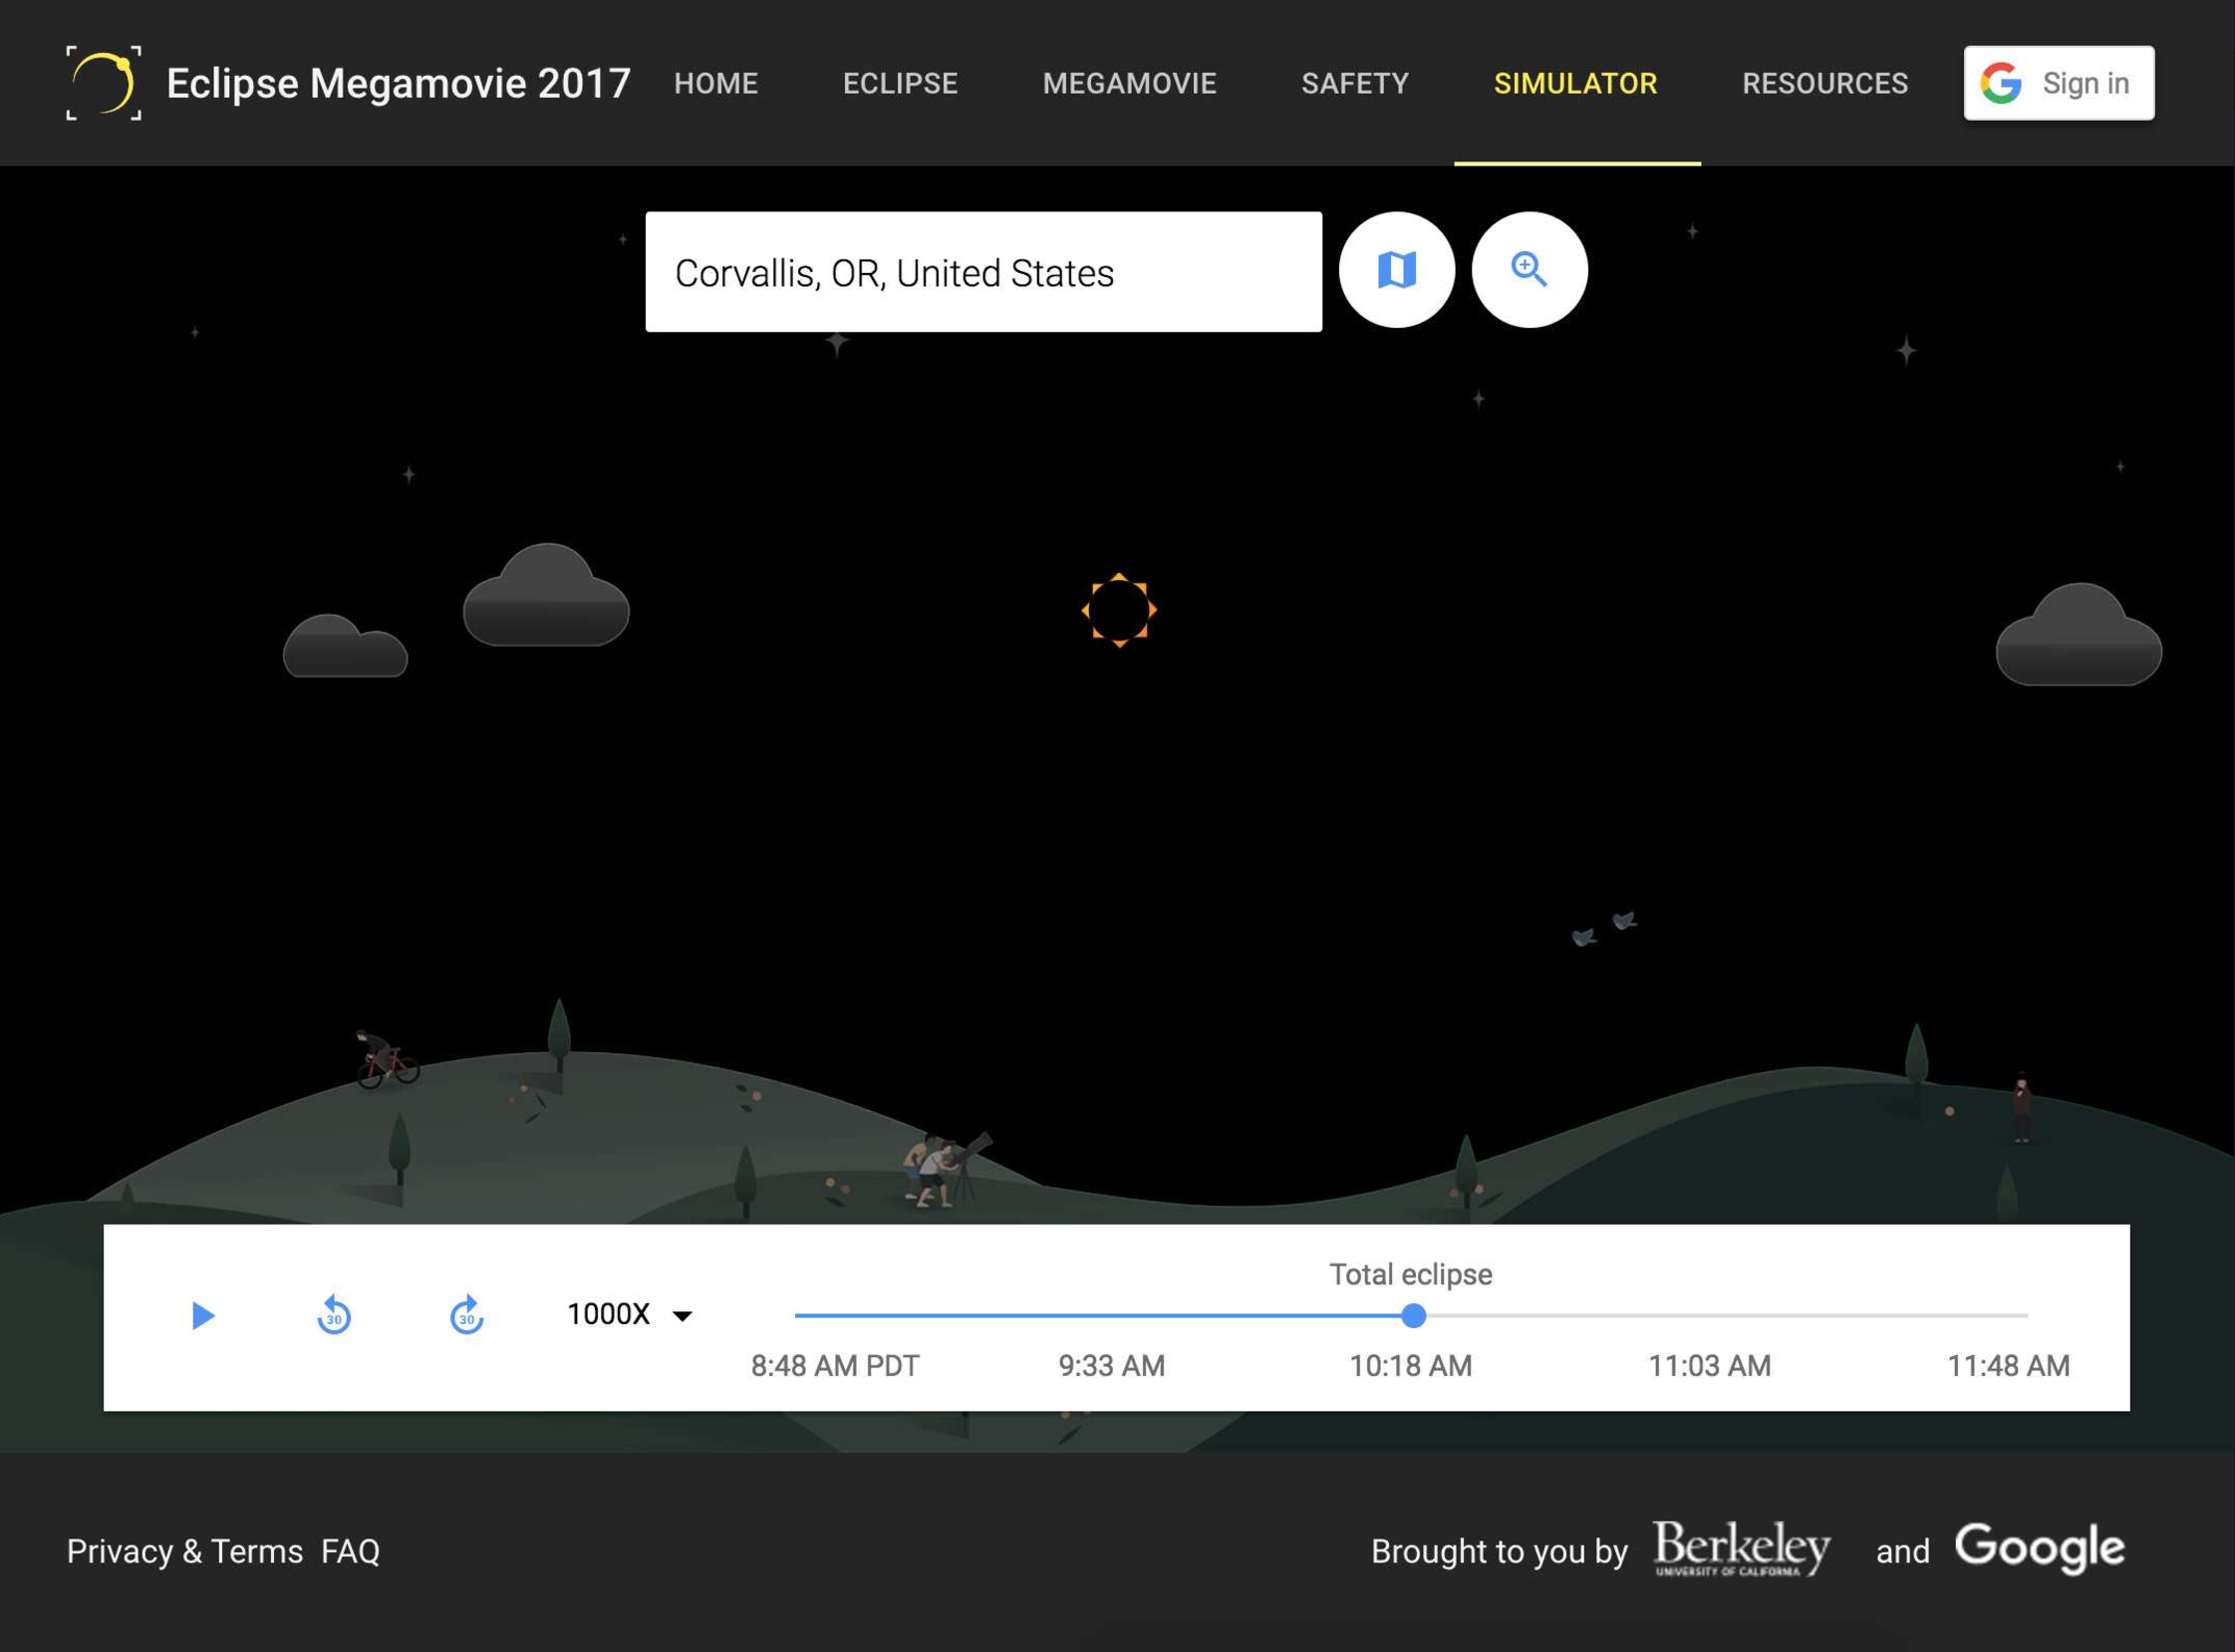
\includegraphics[width=\textwidth]{sim_total.pdf}
		\caption{Simulator in wide mode showing a total solar eclipse}
	\end{center}
\end{figure}
\newpage

\begin{figure}[!h]
	\begin{center}
			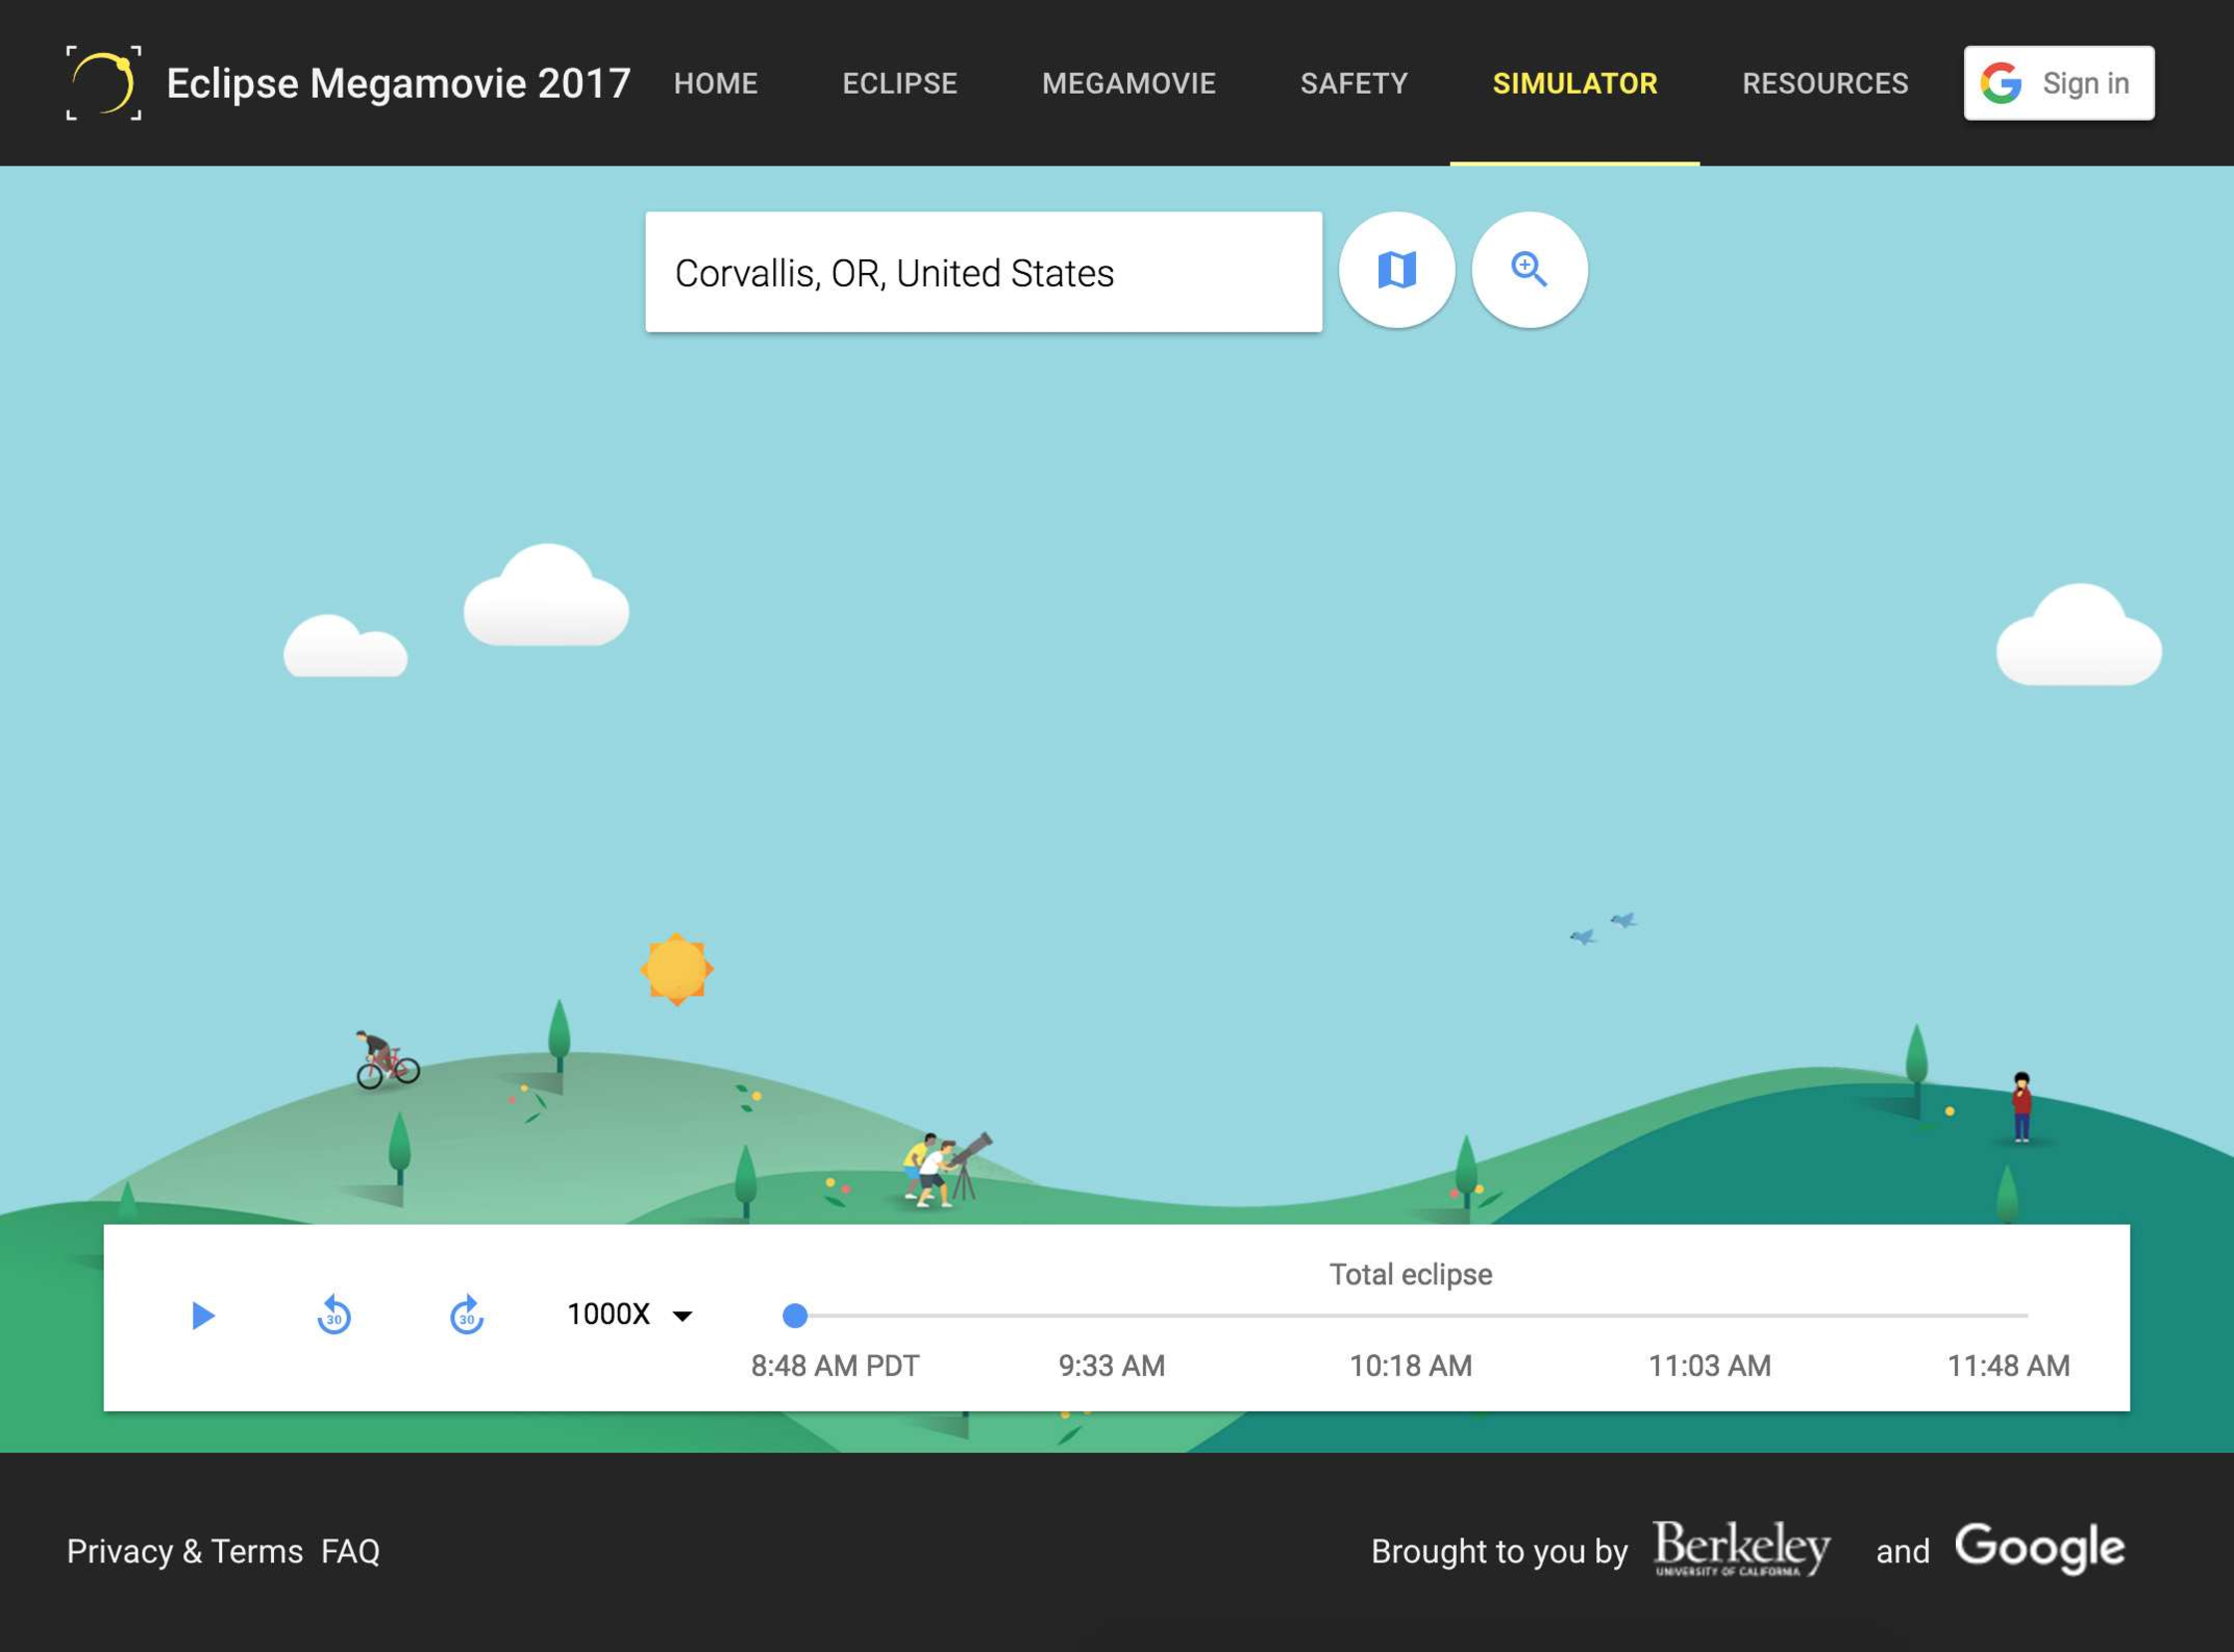
\includegraphics[width=\textwidth]{sim.pdf}
		\caption{Simulator in wide mode showing no eclipse}
	\end{center}
\end{figure}
\newpage

\begin{figure}[!h]
	\begin{center}
			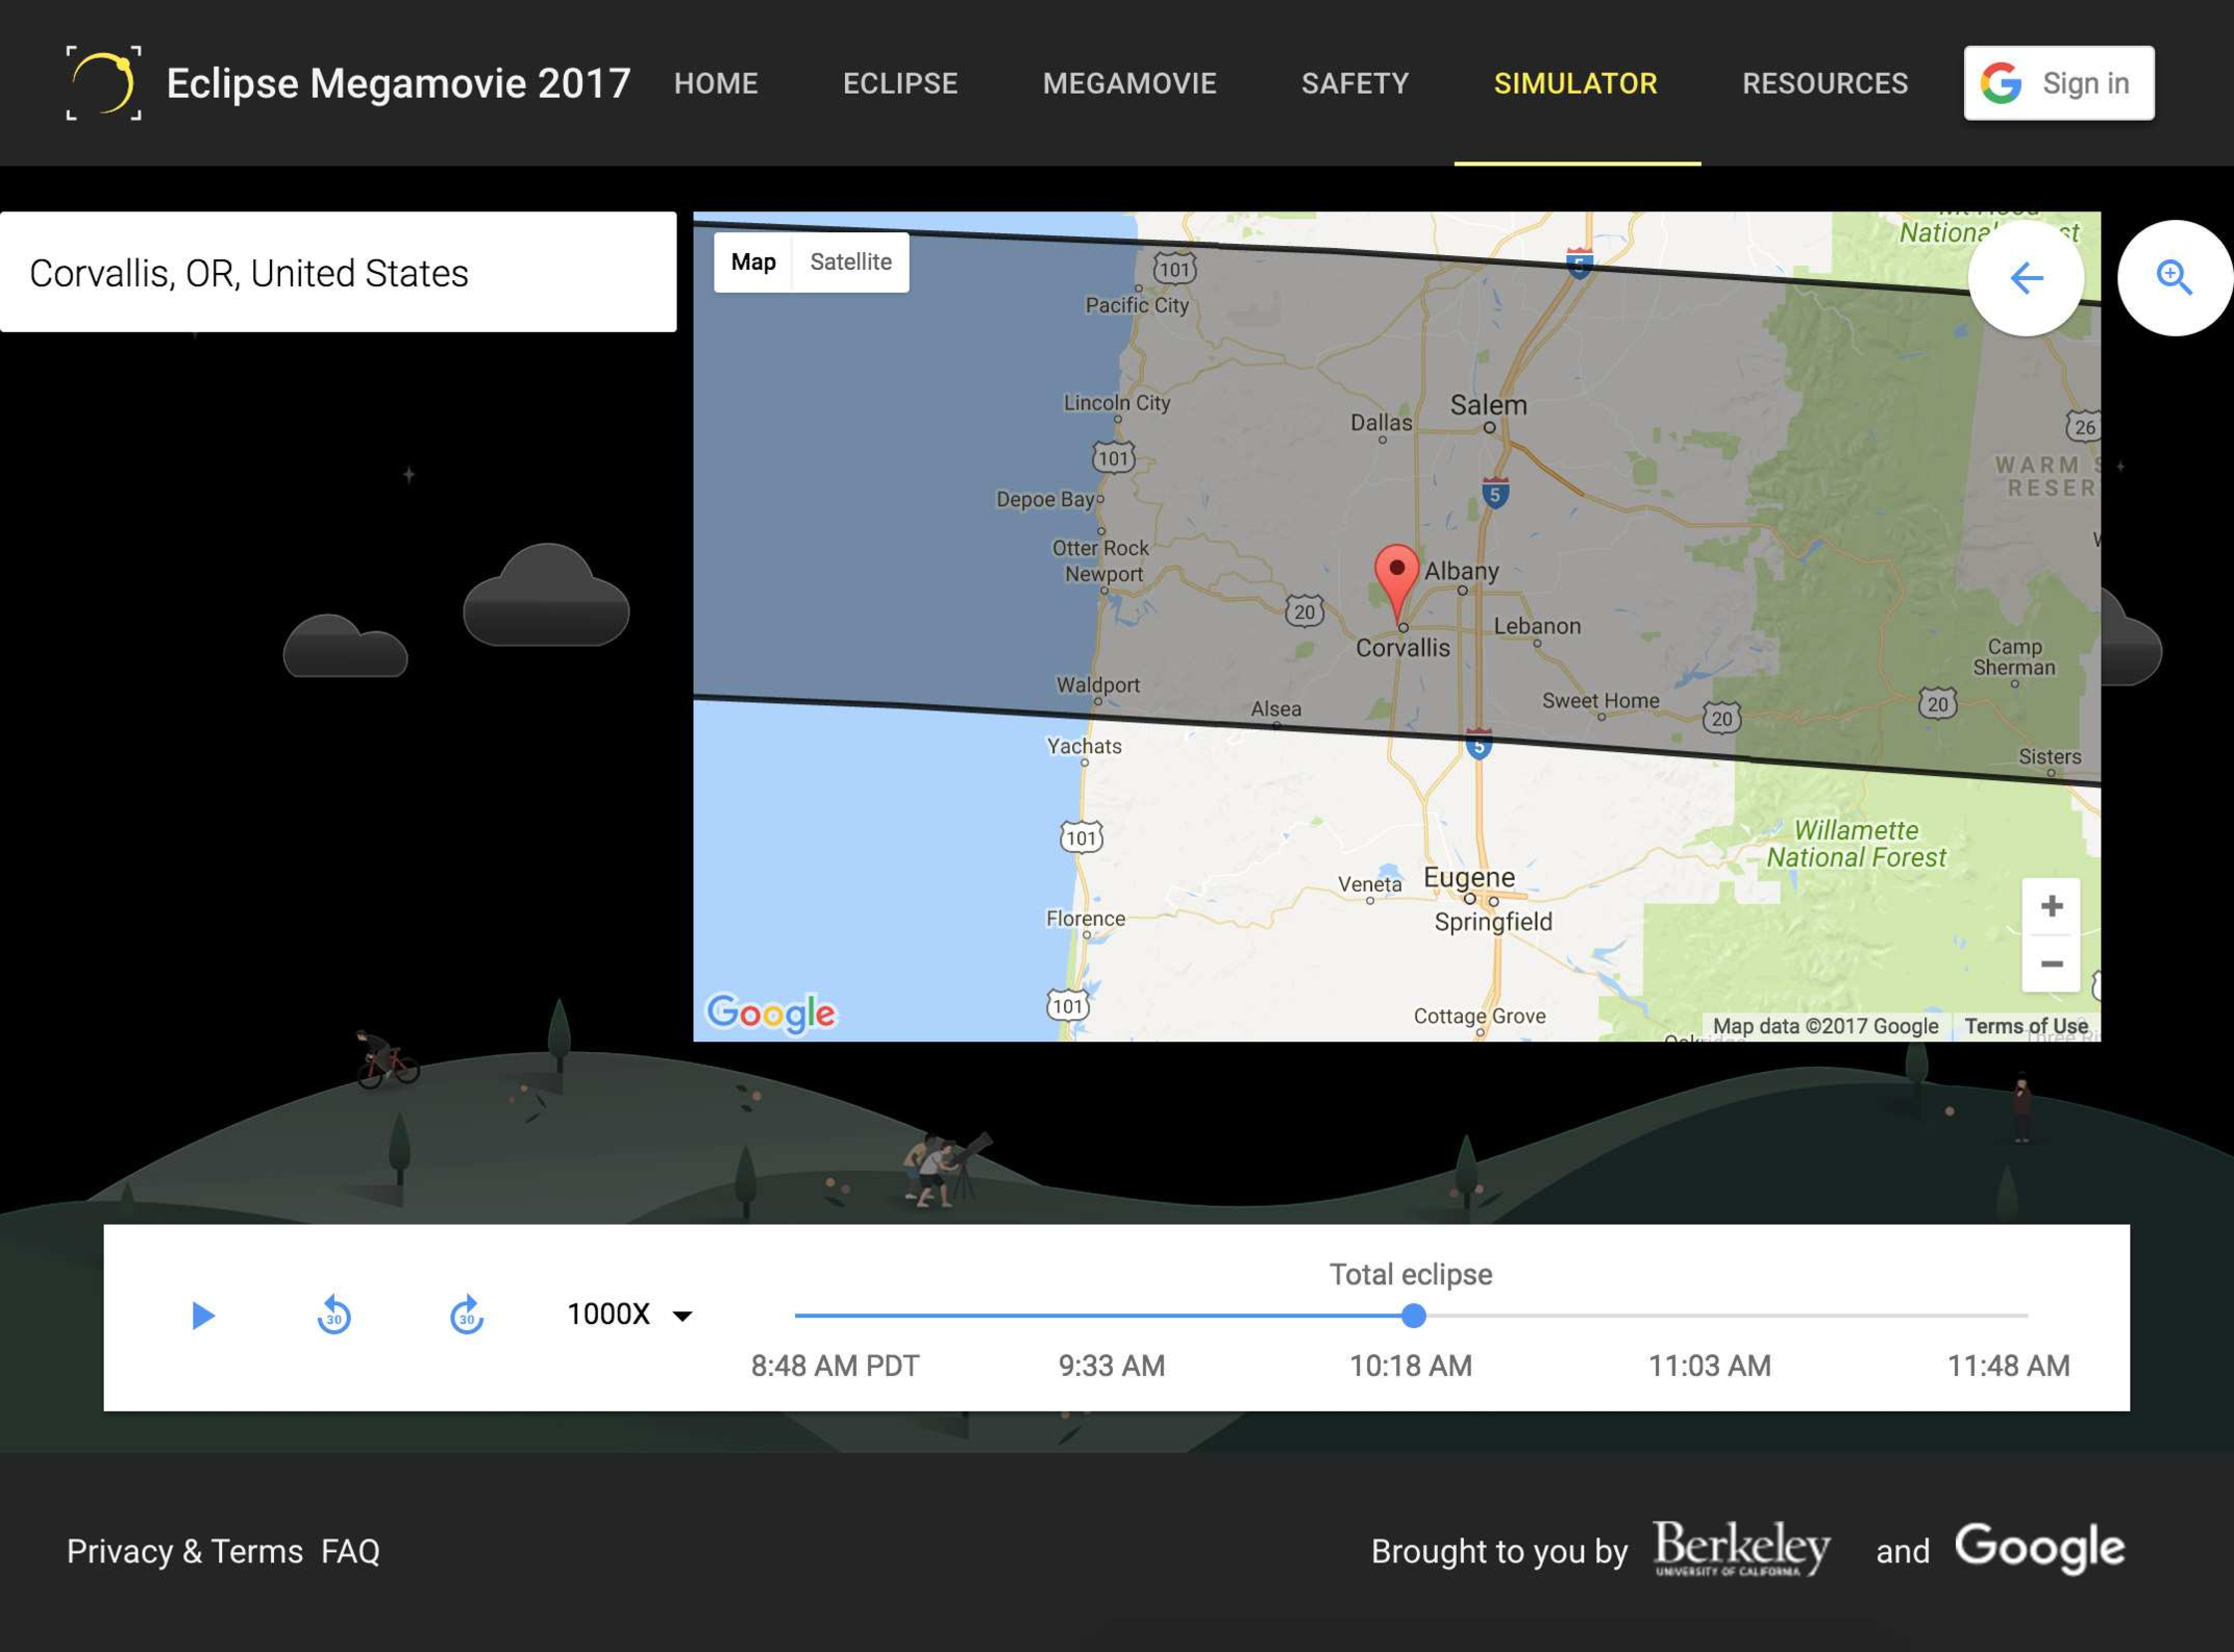
\includegraphics[width=\textwidth]{sim_map.pdf}
		\caption{Simulator with map expanded}
	\end{center}
\end{figure}
\newpage

\begin{figure}[!h]
    \begin{center}
            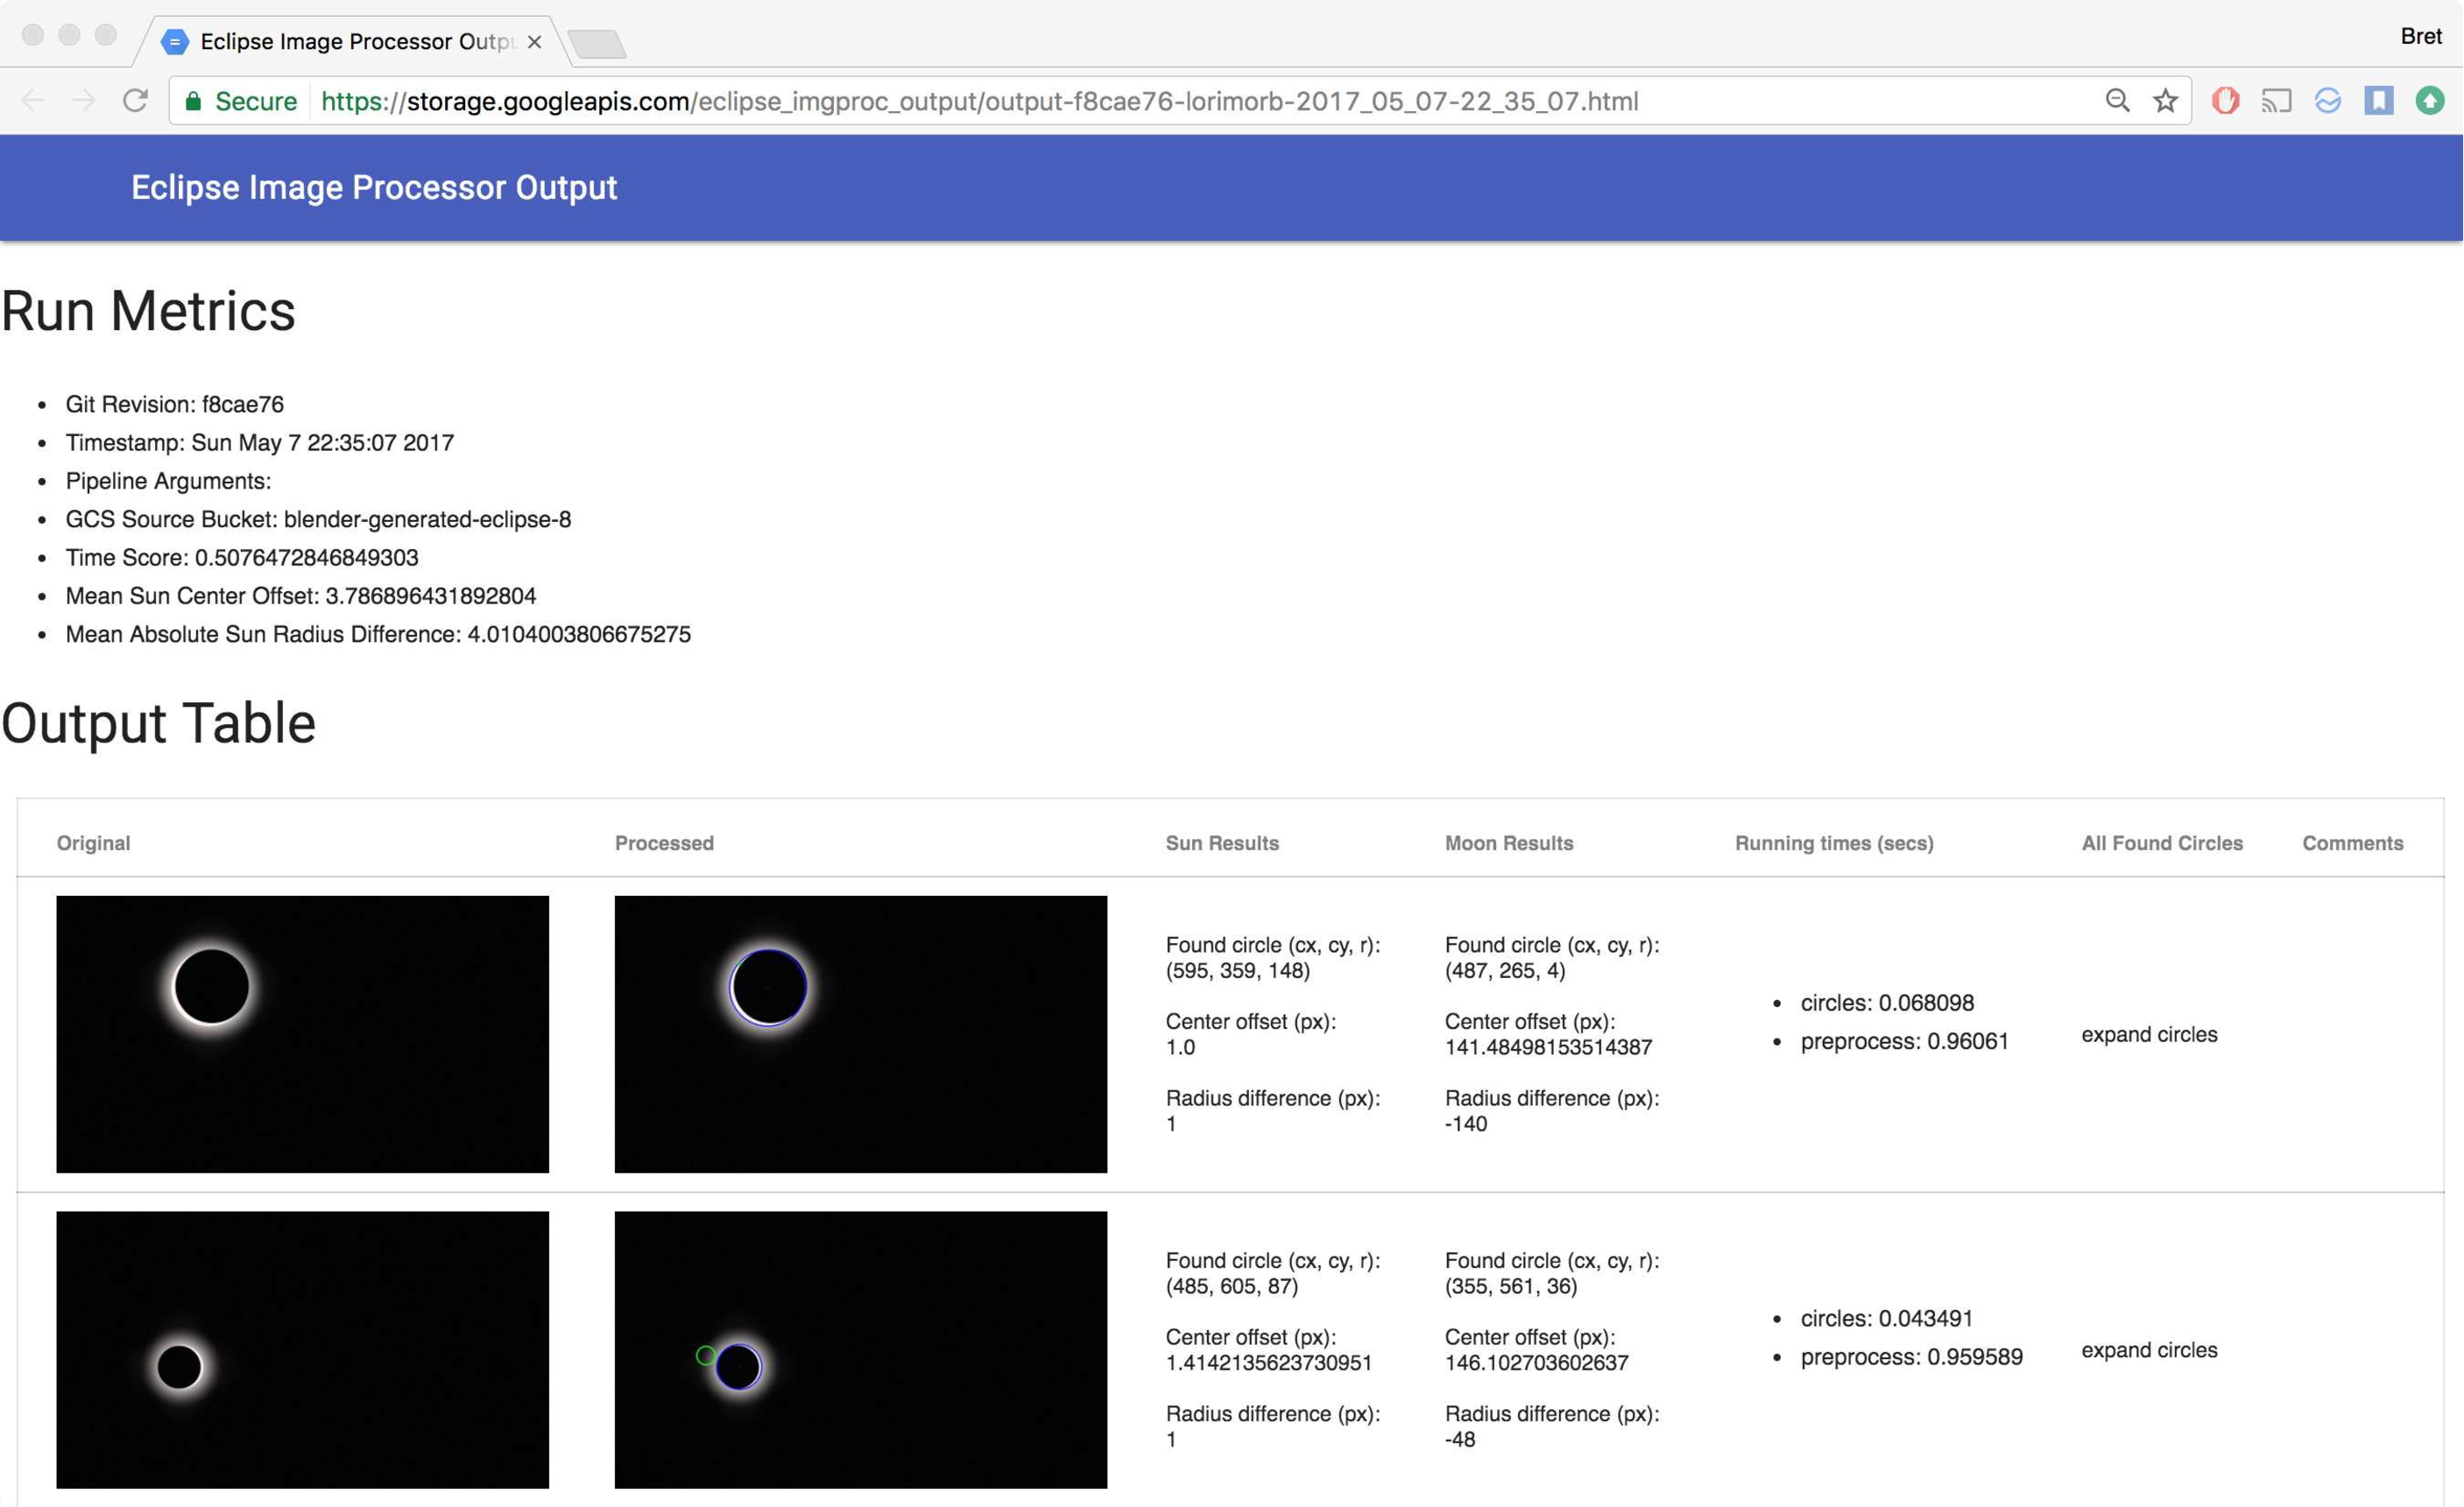
\includegraphics[width=\textwidth]{imgproc.pdf}
        \caption{Image Processor Developer Pipeline Results File}
    \end{center}
\end{figure}
\newpage

\end{document}
